\documentclass[11pt]{article}

% Language setting
% Replace `english' with e.g. `spanish' to change the document language
\usepackage{babel}

% Set page size and margins
% Replace `letterpaper' with `a4paper' for UK/EU standard size
\usepackage{geometry}

% Useful packages
\usepackage{multirow}
\usepackage{subfloat}
\usepackage{stfloats}
\usepackage{float}
\usepackage{subfig}
\usepackage{subcaption}
\usepackage{caption}
\usepackage{amsmath}
\usepackage{hyperref} 
\usepackage{graphicx} 
\usepackage{hyperref}
\usepackage{algorithm}
\usepackage{algorithm2e}
\usepackage{amsthm}
\usepackage{comment}
\newtheorem{defn}{Definition}
\graphicspath{{MainFolder/}} 

\begin{document}

\title{A Review of Adaptive Techniques and Data Management Issues in DP-SGD}
\author{Islam A. Monir, Muhamad I. Fauzan, Gabriel Ghinita}

\date{}

\maketitle

\begin{abstract}
Differentially-Private Stochastic Gradient Descent (DP-SGD) established itself as the most prominent technique for training neural networks with formal privacy guarantees. Almost a decade after its introduction, DP-SGD has become the de-facto standard for privacy-preserving learning from large datasets with individual records. However, important research and engineering issues remain open to more accurate and efficient solutions. Existing approaches either require large amounts of privacy budget to train accurately, and incur high overheads in terms of computational and memory resources consumption. In this article, we provide a critical review of some of the most prominent DP-SGD approaches, and discuss their relative strengths and weaknesses. Specifically, we look at several adaptive approaches that attempt to improve the privacy-accuracy trade-off during learning, by dynamically adjusting parameters such as clipping threshold, learning rate or budget allocation. We also provide an overview of important data management aspects in DP-SGD, which influence significantly its computational and memory overhead. Finally, we review a novel approach to support heterogeneous privacy requirements, i.e., individualized privacy settings.
\end{abstract}

\section{Introduction}

The past decade witnessed the emergence of machine learning, and in particular neural networks, as the tool of choice for a broad area of application domains, e.g., healthcare, social media, computer vision, cybersecurity, etc. For neural network to perform accurately, large input datasets are required to train them. Often, these datasets consist of individuals' data, e.g., user profiles and purchasing records, patient records, user browsing history, etc., which if not carefully handled, may disclose sensitive data regarding one's health status or personal lifestyle details.

To address individual privacy concerns, differential privacy (DP)~\cite{dworkDP} emerged as the de-facto standard in data protection. The main strength of DP is that it provides formal protection guarantees, and it allows one to derive statistically-significant patterns from large amounts of user-centric data, without allowing an adversary to determine whether the data of any targeted individual has been used or not in the model's training set. In the context of training neural networks, DP has been implemented in conjunction with the popular Stochastic Gradient Descent (SGD) approach, resulting in its privacy-preserving version DP-SGD~\cite{RefWorks:RefID:40-abadi2016deep}. While DP-SGD is a powerful tool, it still presents challenges with respect to the trade-off between privacy and utility of learned models, as well as a number of performance concerns. A significant number of research contributions~\cite{RefWorks:RefID:37-andrewdifferentially,chen2020stochastic,RefWorks:RefID:35-pichapati2019adaclip:,RefWorks:RefID:39-he2022exploring,RefWorks:RefID:38-koskelalearning}, focused on how to adapt DP-SGD and tune it such that utility is increased. In this paper, we provide a review of some of the most prominent adaptive DP-SGD approaches, and we also look at several novel techniques that explore personalized individual requirements~\cite{pate,haveit}. In addition, we explore several data management and performance issues that arise when privately training large models using sizeable datasets. Finally, we provide a brief experimental benchmarking of some of the reviewed approaches, with the purpose of comparing their performance head-to-head on common datasets and under similar parameter settings.

The rest of the article is organized as follows: Section~\ref{bckg} presents fundamental concepts and definitions. Adaptive strategies are overviewed in~Section~\ref{sec:adaptation}. Section~\ref{sec:mgmt} focuses on data management and performance issues in DP-SGD. 
Section~\ref{sec:individ} looks at approaches for individualized privacy constraints. We perform a comparative experimental analysis of some of the considered approaches in Section~\ref{sec:exps} to better understand their relative performance, followed by conclusions in Section~\ref{sec:conclusions}.

\section{Background}
\label{bckg}

\subsection{Differential Privacy}

Dalenius' 1977 principle for statistical databases aimed to ensure individual privacy \cite{dalenius1977towards}, but achieving it akin to semantic security turned out to be impossible, posing risks even to those not included in the database. More recently, Differential Privacy (DP) emerged as the preferred model for quantifying the added privacy risks for datasets of individual records.
The concept of differential privacy was first introduced by Dwork et al. \cite{dworkDP}, who provided a mathematical framework for quantifying the privacy guarantees provided by a given algorithm. 
\\
    Differential privacy ensures that attackers cannot discriminate between any two ``sibling'' inputs by looking at query outputs even when taking into account arbitrary background information. It was proposed in order to offer a statistical guarantee that publicly available aggregate data would not disclose the identity of any individual from the dataset. The exact definition of sibling datasets is provided by the neighboring concept, which in machine learning is best-defined as the neighboring relationship on unstructured data as follows. %Put differently, there is a near probability that a published statistical result comes from two possible datasets \cite{DPSurvey}. 
%The definition of neighboring databases for the two possible datasets is as follows.

\begin{defn}[Neighboring Unstructured Data]\label{def:neighboring}
    Two unstructured datasets $[US]_i$ and $[US]_j$ are said to be neighboring if the Hamming distance between their aggregated real-valued data representations $x_i$ and $x_j$ is at most $m$ \cite{DPSurvey}, where $m$ is the maximum allowed difference, typically set to 1:
    \[ d(x_i, x_j) \leq m \]
\end{defn}


\\
Assume we have two neighboring datasets, $D_1$ and $D_2$, that differ only by a single data item. When we interact with the data via a randomized mechanism $M$, we say that $M$ is $\epsilon$-differentially private if the probability of observing a given output of $M$ does not vary by more than exp($\epsilon$) between any two input different datasets, where $\epsilon$ is defined as the privacy budget. 

\begin{defn}[$\epsilon$-Differential Privacy \cite{DPSurvey,DPSurvey2}]
A randomized mechanism $M$ satisfies $\epsilon$-differential privacy if for every output $S \subseteq \text{range}(M)$ and for all $D_1 \sim D_2 \in \mathcal{D}^n$, the following holds:

\[
\Pr[M(D_1) \in S] \leq \exp(\epsilon) \cdot \Pr[M(D_2) \in S].
\]
\end{defn}


The indistinguishability constraint has later been relaxed to include a $\delta$ additive term, changing the definition to ($\epsilon, \delta$)- differentially privacy. The additional parameter allows for a very small probability (bounded by $\delta$) that the algorithm might deviate from the strict privacy guarantee of $\varepsilon$, providing a trade-off between privacy and accuracy. %This slightly modifies the original equation to become: 
\begin{defn}[$(\epsilon, \delta)$-Differential Privacy \cite{concentrated,chen2020stochastic}]
A randomized mechanism $M$ satisfies $(\epsilon, \delta)$-differential privacy if for every output $S \subseteq \text{range}(M)$ and for all $D_1 \sim D_2 \in \mathcal{D}^n$, the following holds:

\[
\Pr[M(D_1) \in S] \leq \exp(\epsilon) \cdot \Pr[M(D_2) \in S] + \delta.
\]
\end{defn}

The Gaussian mechanism is a noise-addition mechanism that satisfies $(\epsilon,\delta)$-DP (for $\delta > 0$). Through this approach, the $L_2$ sensitivity of the query function is adjusted with Gaussian noise \cite{concentrated}.

\begin{defn}[$L_2$ Sensitivity~\cite{concentrated}]
Let $f: \mathcal{X}^n \rightarrow \mathbb{R}^d$ be a query function. The $L_2$ sensitivity of $f$, denoted by $\Delta_2(f)$, is defined as:
\[
\Delta_2(f) = \max_{X \sim X'} \| f(X) - f(X') \|_2
\]
\end{defn}

\begin{defn}[Gaussian Mechanism~\cite{concentrated}]
For any arbitrary $\epsilon$ from the interval $(0, 1)$ and a query function $q$ with $L_2$ sensitivity $\Delta_2(q)$, the Gaussian Mechanism ensures $(\epsilon, \delta)$-differential privacy. This mechanism adds Gaussian noise $N(0, \sigma^2)$ to $q(D)$, where $\sigma$ satisfies 
\[ \sigma \geq \frac{\Delta_2(q)}{\epsilon} \sqrt{2 \ln\left(\frac{1.25}{\delta}\right)} \]

\end{defn}

Another variation of the differential privacy definition is Rényi Differential Privacy (RDP) \cite{mironov2017renyi}. A generalization of the Kullback-Leibler divergence \cite{kullrenyi}, Rényi divergence serves as the foundation for RDP. Conventional DP quantifies the privacy guarantee by means of the privacy loss parameter $\epsilon$, which limits the probability ratio of a mechanism's outputs in the presence of two adjacent datasets. Conversely, RDP offers a more flexible and fine-grained measure of privacy by including a parameter, $\alpha$ (the order of Rényi divergence), in addition to $\epsilon$.

\begin{defn}[Rényi Divergence \cite{chen2020stochastic,mironov2017renyi}]
For two probability distributions $P$ and $Q$ and a parameter $\alpha > 1$,  the Rényi divergence of order $\alpha$ is defined as:
\[
D_{\alpha}(P \| Q) = \frac{1}{\alpha - 1} \log \left( \sum_{x} P(x)^{\alpha} Q(x)^{1-\alpha} \right)
\]
\end{defn}

\begin{defn}[Rényi Differential Privacy \cite{chen2020stochastic,mironov2017renyi}]
A randomized mechanism $\mathcal{M}$ is said to be $(\alpha, \epsilon)$-RDP if for any two neighboring datasets $D_1$ and $D_2$:
\[
D_{\alpha}(\mathcal{M}(D_1) \| \mathcal{M}(D_2)) \leq \epsilon
\]
\end{defn}

In differential privacy, tracking the cumulative privacy loss, or privacy budget, is crucial, particularly in scenarios involving multiple applications or complex compositions of privacy mechanisms. Traditional methods often struggle to provide tight and accurate bounds on this cumulative privacy loss. To address this, a sophisticated method known as the Moments Accountant ($MA$) has been developed. The $MA$ leverages the framework of Rényi Differential Privacy (RDP) to achieve precise tracking of the privacy budget. By calculating the moments, or expected values of powers, of the privacy loss random variable, it quantifies the degradation of privacy guarantees over successive computations. This method utilizes RDP to evaluate the Rényi divergence between the output distributions of the mechanism for neighboring datasets at each step, allowing for a more refined and accurate assessment of the privacy-utility trade-off. 
%It is more often used with Differentially Private Stochastic Gradient Descent (discussed in section \ref{dpsgdsec}) and is discussed more in the work done by Abadi et. al. \cite{RefWorks:RefID:40-abadi2016deep}


\subsection{Differentially Private Stochastic Gradient Descent (DP-SGD)}
\label{dpsgdsec}
Stochastic Gradient Descent (SGD) is a popular optimization technique employed in the training of machine learning models. SGD iteratively adjusts model parameters by leveraging the gradients of a loss function, which are computed based on a randomly selected subset of the training data, known as a batch \cite{gower2019sgd,tian2023recent}. The specific rule for updating the model parameters is given by:

\[
\theta_{t+1} = \theta_t - \eta \nabla J(\theta_t; x^{(i)}, y^{(i)})
\]

where \(\theta_t\) denotes the model parameters at iteration \(t\), \(\eta\) is the learning rate, and \(J(\theta_t; x^{(i)}, y^{(i)})\) represents the loss function evaluated on the current batch \((x^{(i)}, y^{(i)})\).

DP-SGD extends Stochastic Gradient Descent (SGD) to provide differential privacy guarantees while training machine learning models on sensitive data. In DP-SGD, gradient clipping is performed before adding noise to the gradients to ensure that the gradients remain bounded.

The clipped gradient \( \hat{\nabla} f(\theta, D_t) \) for one sample of data \( D_t \) is computed as:
\[ \hat{\nabla} f(\theta, D_t) = \text{Clip}(\nabla f(\theta, D_t), C) \]
where:
\begin{itemize}
\item \( \nabla f(\theta, D_t) \) is the gradient of the loss function with respect to the model parameters \( \theta \) computed on data sample \( D_t \),
\item \( C \) is the clipping threshold, which limits the magnitude of the gradients.
\end{itemize}

Clipping plays a pivotal role in the DP-SGD process in balancing the trade-off between privacy and utility. Clipping the gradients is needed to prevent outliers (extreme or unusually large gradients) and it limits their sensitivity, preventing the model from learning more than a set quantity from any given sample, which prevents inadvertent leakage of information during training and thus satisfies differential privacy. It is important to note that the way clipping is performed can vary, and the method of clipping can end up affecting the algorithms performance. In the original implementation of DP-SGD done by Abadi et. al.~\cite{RefWorks:RefID:40-abadi2016deep}, a random sample from a mini-batch is used to compute gradients. For each sample gradient, a check is performed to see if the magnitude of the gradient is larger than the clipping threshold. If the magnitude of the gradient is determined to be greater than the clipping threshold, it gets scaled down to its $L_2$ norm $C$ as follows:
\[ \Bar{g}_t \leftarrow g_t(x_i)/\text{max}(1,\frac{||g_t(x_i)||_2}{C})\]
where $\text{max}(1,\frac{||g_t(x_i)||_2}{C})$ is the maximum value between $1$ and the magnitude of the gradient divided by the clipping threshold. If the magnitude of the gradient is less than the clipping threshold, the gradient would end up being divided by 1, thus preserving the original gradient. If the gradient is larger than the clipping threshold $C$, the value of $||g_t(x_i)||_2$ will ends up being greater than 1, and the original gradient is divides to scale it down to the clipping threshold.

After clipping the gradients, noise is added to ensure differential privacy:
\[ \tilde{\nabla} f(\theta, D_t) = \hat{\nabla} f(\theta, D_t) + \mathcal{N}(0, \sigma C I_n) \]
where:
\begin{itemize}
\item \( \mathcal{N}(0, \sigma C I_n) \) is the noise term drawn from the Gaussian distribution with mean \( 0 \) and scale parameter \( \sigma C I_n \),
\item \( \epsilon \) is the privacy parameter, controlling the privacy strength.
\end{itemize}

After adding noise to the clipped gradients, the model parameters are updated using the noisy gradients:
\[ \theta_{t+1} = \theta_{t} - \eta \tilde{\nabla} f(\theta, D_t) \]

The use of privacy budgets is a crucial component of DP-SGD. Because SGD is iterative, if one applies the traditional sequential composition theorem \cite{gong2020survey}, which states that the total budget for the learning process is equal to the sum of the budgets used in each iteration, the budget consumption can increase significantly. The moments accountant ($MA$)  introduced in~\cite{RefWorks:RefID:40-abadi2016deep} offers a tighter bound on privacy budget consumption using Poisson sampling.

The trade-off between privacy and utility in DP-SGD encapsulates the delicate balance between preserving the privacy of sensitive data and maintaining the effectiveness of the trained machine learning model. DP-SGD introduces noise to the gradients during the training process to ensure that individual data points do not unduly influence the model updates, thereby providing strong privacy guarantees. However, this noise addition can degrade the quality of the learned model, leading to a reduction in its performance on the task at hand. Figures \ref{fig:sgd} and \ref{fig:dpsgd} illustrate the difference in the algorithm structure between SGD and DP-SGD.

\begin{figure}[h]
\centering
    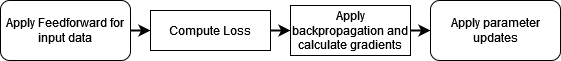
\includegraphics[width=0.7\linewidth]{submissions/submission5/figs/sgd.drawio.png}
   \caption{Conventional (non-private) SGD workflow}
   \label{fig:sgd}
\end{figure} 
\begin{figure}[h]
\centering
    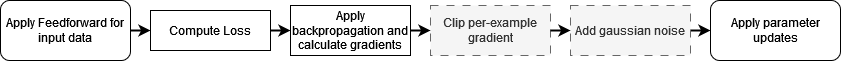
\includegraphics[width=1\linewidth]{submissions/submission5/figs/dpsgd.drawio.png}
   \caption{DP-SGD workflow}
   \label{fig:dpsgd}
\end{figure} 

\iffalse
\subsection{Gradient Clipping Parameter}
(Content to be moved to Data Management Section)
Clipping plays a pivotal role in the DP-SGD process in balancing the trade-off between privacy and utility. Clipping the gradients is needed to prevent outliers (extreme or unusually large gradients) and such limits their sensitivity, meaning we prevent the model from learning more than a set quantity from any given sample, which prevents inadvertent leakage of information during training and preserving the privacy guarantee provided by differential privacy. This bound in the gradient becomes a parameter that is called the clipping threshold. It is important to note that the way clipping is performed can vary from each DP-SGD model, and the method of clipping can end up affecting the algorithms performance. In the original implementation of DP-SGD done by Abadi .et .al\cite{RefWorks:RefID:40-abadi2016deep}, they first take a random sample from a mini-batch and compute the gradient of each sample. Each sample gradient, a check is performed to see if the magnitude of the gradient is larger than the clipping threshold. If the magnitude of the gradient is determined to be greater than the clipping threshold, it gets scaled down to norm $C$. This is given in the equation:
\[ \Bar{g}_t \leftarrow g_t(x_i)/\text{max}(1,\frac{||g_t(x_i)||_2}{C})\]
Where $\text{max}(1,\frac{||g_t(x_i)||_2}{C})$ gets the maximum value between 1 and the magnitude of the gradient divided by the clipping threshold. if the magnitude of the gradient is less than the clipping threshold, the gradient would end up being divided by 1, thus preserving the original gradient. If the gradient is larger than the clipping threshold $C$, the value of $||g_t(x_i)||_2$ will end up being greater than 1, thus making the original gradient divide with the clipped value in order to scale down the gradient by the clipping threshold. This kind of clipping is referred to as $l_2$ norm clipping, where the $l_2$ norm is synonymous with the gradient magnitude.

One significant drawback of DP-SGD lies in its perceived computational expense, primarily attributed to the process of clipping per-example gradients. The instantiation and subsequent potential clipping of these gradients are recognized to impose substantial memory and time costs within standard machine learning frameworks. Consequently, private machine learning using DP-SGD is frequently observed to exhibit slower performance and greater computational demands compared to its non-private counterparts. Author He et. al\cite{RefWorks:RefID:39-he2022exploring} suggests there are mainly two different per-example gradient clipping strategies in DP optimization:

Flat Clipping, as initially introduced by Abadi et al. in their original implementation of DP-SGD, presents a foundational clipping schema discussed earlier. However, a notable limitation of this schema arises: flat clipping necessitates gradient norms computation before it can be applied. This sequential requirement mandates the completion of backpropagation first, adding an extra computational step post-backpropagation solely for the purpose of clipping. Consequently, this approach introduces additional overhead, particularly problematic when dealing with models whose weights exceed the capacity of a single device—a common occurrence, especially with larger models.
Group-Wise clipping was the other schema described that involved partitioning the set of parameters $\theta$ into $K$ disjoint groups. The main idea in group-wise clipping is that each group would have its own clipping threshold, where the gradient within that group is clipped separately. In certain cases, the gradients would be divided into groups based on the layers of the neural network.

We'll begin by exploring per-layer clipping, a form of group-wise clipping that assigns specific clipping thresholds to individual layers within a neural network. In this approach, each of the $K$ layers in the network is assigned its own threshold, denoted as $C_k$, for clipping the gradients of that layer. One notable advantage of per-layer clipping is its immediate applicability—gradient clipping can be performed as soon as backpropagation reaches each layer, unlike flat clipping, which necessitates completion of the entire backpropagation process. Experimental results with per-layer clipping have demonstrated its ability to closely match the memory profile and training throughput of non-private models, proving it to be computationally efficient compared to flat clipping.
Although per-layer clipping offers computational advantages over flat clipping, it has been reported to exhibit lower accuracy performance in certain scenarios. For instance, when tested on a randomly sampled set of CIFAR-10 examples for privately training WRN16-4, per-layer clipping yielded a validation accuracy of 60.6\%, compared to the 63.1\% achieved with flat clipping (with a privacy budget set to $\varepsilon$ = 3). Observations during training reveal significant fluctuations in the magnitudes of per-layer gradients throughout the process. While gradients may initially be uniformly low, they tend to increase notably for layers closer to the input as training progresses. It is suggested that employing a fixed layer-wise clipping threshold eliminates the structural relationship between gradients of different layers, introducing an additional source of bias on top of the inherent bias associated with flat clipping techniques.

A solution to the performance problems of fixed per-layer clipping is to introduce adaptive clipping thresholds in the hopes of removing the structural bias that comes with clipping gradients of different layers separately. This is mainly done through quantile estimation. Some percentage of the total privacy budget ($r=1\%$ to 10\% of total budget) is allocated for estimating the target quantile for each layer’s gradient norms. The clipping threshold for each layer $C_1,...,C_K$ is then set to the estimated quantiles. The number of gradients clipped in each layer are recorded before each parameter update, and the clipping threshold is then adjusted based on whether too few or too many gradients have been clipped. The fraction of clipped gradients needs to be privatized, and an additional noise multiplier is added to achieve this goal. This addition also affects the noise multiplier for noising parameter updates, and the new noise multiplier is calculated from:
\[ \sigma_\text{new}=(\sigma^{-2}-K(2\sigma_b)^2)^{-1/2}\]
Where $\sigm_b$ is the additional noise multiplier for the privatized clipped fraction, σ is the original noise multiplier and $K$ is the number of layers in the neural network (also known as number of groups).
\fi

\section{Adaptive DP-SGD Approaches}
\label{sec:adaptation}
The performance of ML algorithms is highly-dependent on the properties of the data. In the case of private learning, the constraints imposed by DP create additional challenges, and hence having fixed parameter settings is even less likely to perform well, leading to low accuracy or high privacy budget consumption (i.e., low protection). A significant amount of research explored the idea of adapting parameter values to the training data, or to other inputs such as number of iterations, batch size, privacy budget, learning rate, etc.~\cite{RefWorks:RefID:35-pichapati2019adaclip:,RefWorks:RefID:38-koskelalearning,RefWorks:RefID:48-fay2023adaptive}. %Typically, parameter values change at each step to fit the current iterations requirement. 

%Although we have only briefly discussed the idea of adaptive clipping in subsection 3.2.1, other parameters are also beings considered for adaptivity, including the learning rate and the privacy budget. 
In this section, we review several adaptive DP-SGD approaches, which fall mainly into three categories: tuning the privacy budget over time, varying the clipping threshold, or changing the learning rate. Adjusting these parameters offers several advantages. For instance, once can directly control the privacy budget consumption, which in DP-SGD is an output of the noise injection procedure (whereas the input is represented by noise magnitude). Furthermore, the privacy/accuracy trade-off of DP-SGD~\cite{RefWorks:RefID:47-yu2019differentially} can be better controlled, as hyperparameter values can significantly affect the performance of trained models~\cite{RefWorks:RefID:39-he2022exploring}. However, in the case of private learning, selecting optimal hyperparameter values is a lot more challenging than in non-private learning, due to the fact that any information used in tuning them has to be itself sanitized, potentially leading to additional privacy budget consumption. In contrast, with non-private learning, one can rely on trial-and-error approaches to do an exhaustive search of the hyperparameter space. Although some existing works have explored the problem or private hyperparameter tuning, they typically do not guarantee optimality of parameters, and they often increase the privacy budget consumed~\cite{RefWorks:RefID:52-liu2019private}.
 
\subsection{Privacy Budget Adaptation}
\label{secPri}
Perhaps the most challenging task in DP-SGD is striking a good trade-off between privacy and utility. DP-SGD injects noise into the gradient values during the training process to ensure that individual data points do not significantly influence the model updates in a way that allows re-identification. However, the noise addition process also degrades the quality of the learned model, leading to a reduction in its performance on the task at hand~\cite{RefWorks:RefID:40-abadi2016deep}. Hence, a delicate balance must be achieved between preserving the privacy of sensitive data and maintaining the effectiveness of the trained machine learning model. Next, we review three directions in which this trade-off can be controlled.



\subsubsection{Noise Decay}
\label{decay}

The first study that addressed adapting the DP-SGD privacy budget~\cite{RefWorks:RefID:47-yu2019differentially} proposed a solution based on the idea that, as the model converges, the gradient is expected to have a lower magnitude, thus allowing the learning process to converge faster to a local optimal, and achieve higher accuracy. To this end, a set of methods for privacy budget allocation were defined in~\cite{RefWorks:RefID:47-yu2019differentially} that dynamically reduce the noise scale as the training time increases. 
\begin{itemize}
    \item \textbf{Adaptive Schedule Based on Public Validation Dataset:} 
As mentioned earlier, one challenging aspect when making data-dependent decisions with private algorithms is that one must consume privacy budget when accessing any data-derived intermediate results. When public datasets are available, this challenge is averted, as one does not need to protect the inputs of the parameter tuning strategy algorithm. 

    The main idea in this approach is to continuously check the validation error on the {\em public} dataset while training on the private one, and dynamically reduce the noise scale whenever the validation accuracy improves by less than a set threshold $\delta$. In such cases, the noise scale is reduced by a factor of $k$ and this continues until the total privacy budget is consumed.
    %In their proposal, a public validation dataset is used to periodically assess the validation accuracy throughout the training process to ascertain whether the noise scale should be diminished for subsequent epochs. 
The evaluation intervals where validation is carried out are termed {\em validation epochs}.

Let $\sigma_e$ denote the noise scale for the DP-SGD training in validation epoch $e$, and $S_e$ represent the corresponding validation accuracy. The adjustment of the noise scale for subsequent epochs is contingent upon the discrepancy in accuracy between the current epoch $e$ and the preceding validation epoch $e - 1$. Initially, $S_0 = 0$.

The formula for adjusting the noise scale is:

\[
\sigma_e = \begin{cases} 
k \sigma_e, & \text{if } |S - S_{e-1}| \leq \delta \\
\sigma_e, & \text{otherwise} 
\end{cases}
\]

This adjustment ensures that the noise scale adapts based on the performance change observed between validation epochs. If the accuracy difference $S_e-S_{e-1}$ is less than the predetermined threshold $\delta$, the noise scale is attenuated by a factor of $k$ ($0<k<1$). To improve training effectiveness, the moving average of the validation accuracy is considered in the decision process, as there are cases where the validation accuracy does not increase monotonically within the training progress, and any fluctuations may result in unnecessary reduction of noise scale, which in turn consumes privacy budget.

    \item \textbf{Pre-defined Schedules: }
    In cases where a public validation dataset is not available, an alternative solution proposed in~\cite{RefWorks:RefID:47-yu2019differentially} calculates a fixed, data-independent schedule according to which the noise scale decreases over time. Four such decay strategies are presented:

\begin{enumerate}
    \renewcommand{\labelenumi}{\alph{enumi})}
    \item {\em Time-Based Decay}: the noise scale is adjusted using the formula $\sigma_t=\sigma_0/(1+kt)$, where $\sigma_0$ is the initial noise scale, $t$ is the number of training epochs so far, and $k>0$ is the decay rate. When $k<1$, this method is referred to as ``search-then-converge'', and the noise scale decreases linearly during the search phase when $t$ is less than the ``search time'' $1/k$; afterwards, the noise scale decreases by a factor of $1/t$.
    \item {\em Exponential Decay}: The noise scale decreases exponentially with each epoch, according to the expression $\sigma_t=\sigma_0e^{-kt}$, where $k>0$ is the decay rate.
    \item {\em Step Decay}: The noise scale decreases by an exponentially-increasing factor every few epochs, according to expression $\sigma_t=\sigma_0*k^{t/period}$. The decay rate $k$ is chosen such that $0<k<1$.
    \item {\em Polynomial Decay}: The noise parameter follows a polynomial decay function over a specified number of epochs $period$. Specifically,  $\sigma_t=(\sigma_0-\sigma_{end})*(1-t/period)^k+\sigma_\text{end}$ where $k>0$ is the decay rate and $t<period$. When $k=1$, this is referred to as a linear decay function.
\end{enumerate}

\end{itemize}
\subsubsection{Optimal Step Size Search}
\label{sec:step}
The previous approaches looked solely at how to adapt the privacy budget allocation throughout the learning process using different decay functions over time. Next, we look at an approach~\cite{concentrated} that adapts both the privacy budget and the learning rate (while we dedicate a separate section to learning rate adaptation approaches in Section~\ref{sec:lr}, we discuss this hybrid method here).
%The work in~\cite{concentrated} looks at how to find the optimal step based on a given set . B
At the core of the proposed technique from~\cite{concentrated} sits a privacy-preserving algorithm for computing the noisy maximum among the values in a set. The {\em NoisyMax} algorithm   adds independent Laplace noise to each set value and returns the index of the largest one, thereby providing differential privacy guarantees~\cite{concentrated}.

The two main components of the algorithms are {\em step-size selection} and {\em adaptive noise reduction}. The goal of step-size selection is to efficiently choose the per-iteration privacy budget. Adding noise to the gradients may not guarantee the correct direction of the descent, in expectation. To alleviate this issue, a portion of the privacy budget $p_\text{nmax}$ is used to check whether a given noisy estimate $\Tilde{g}_t$ of the gradient gives the correct descent direction. To accomplish this, a set $\Omega=\{f(w_t-\alpha\Tilde{g}_t):\alpha\in\Phi\}$ is constructed, where each element of the set is the objective value evaluated at $f(w_t-\alpha\Tilde{g}_t)$ and $\Phi$ is a set of pre-defined step-sizes. Using the NoisyMax computation, the algorithm calculates which step-size results in the smallest objective function value. Since an a priori bound cannot be determined on a given loss function $l$, gradient clipping is applied to bound sensitivity. This way, the first element of $\phi$ is fixed to $0$, to take into consideration the current objective value. Let $i$ be the index returned by the NoisyMax algorithm. If $i>0$, the algorithm updates $w_t$ using the chosen step size $a_i$. However, if $i=0$, $-\Tilde{g}_t$, it is likely that is not the correct descent direction, and none of the given step sizes will lead to a decrease in the value of the objective function $f$. Hence, the adaptive noise reduction is applied.

A block diagram of the NoisyMax technique is illustrated in Figure~\ref{fig:noisymax}. When the NoisyMax algorithm determines that the current gradient direction is incorrect, the algorithm increases the privacy budget used in noisy gradient approximation by a factor of $1 + y$. Using the gradient averaging technique, a total privacy budget of $p_\text{ng} – p_\text{old}$ is consumed to measure the new gradient with increased accuracy.  The gradient averaging technique is a method that recycles gradient estimates that were not useful by using the difference between two related privacy budget values to measure a new gradient, which when combined with the old measured gradient can be used to measure the final noisy gradient estimate at a lower privacy budget. Once the algorithm measures a new gradient, it goes through the NoisyMax algorithm again to determine its direction. These steps repeat until a good descent direction can be found.

\begin{figure}[h]
\centering
    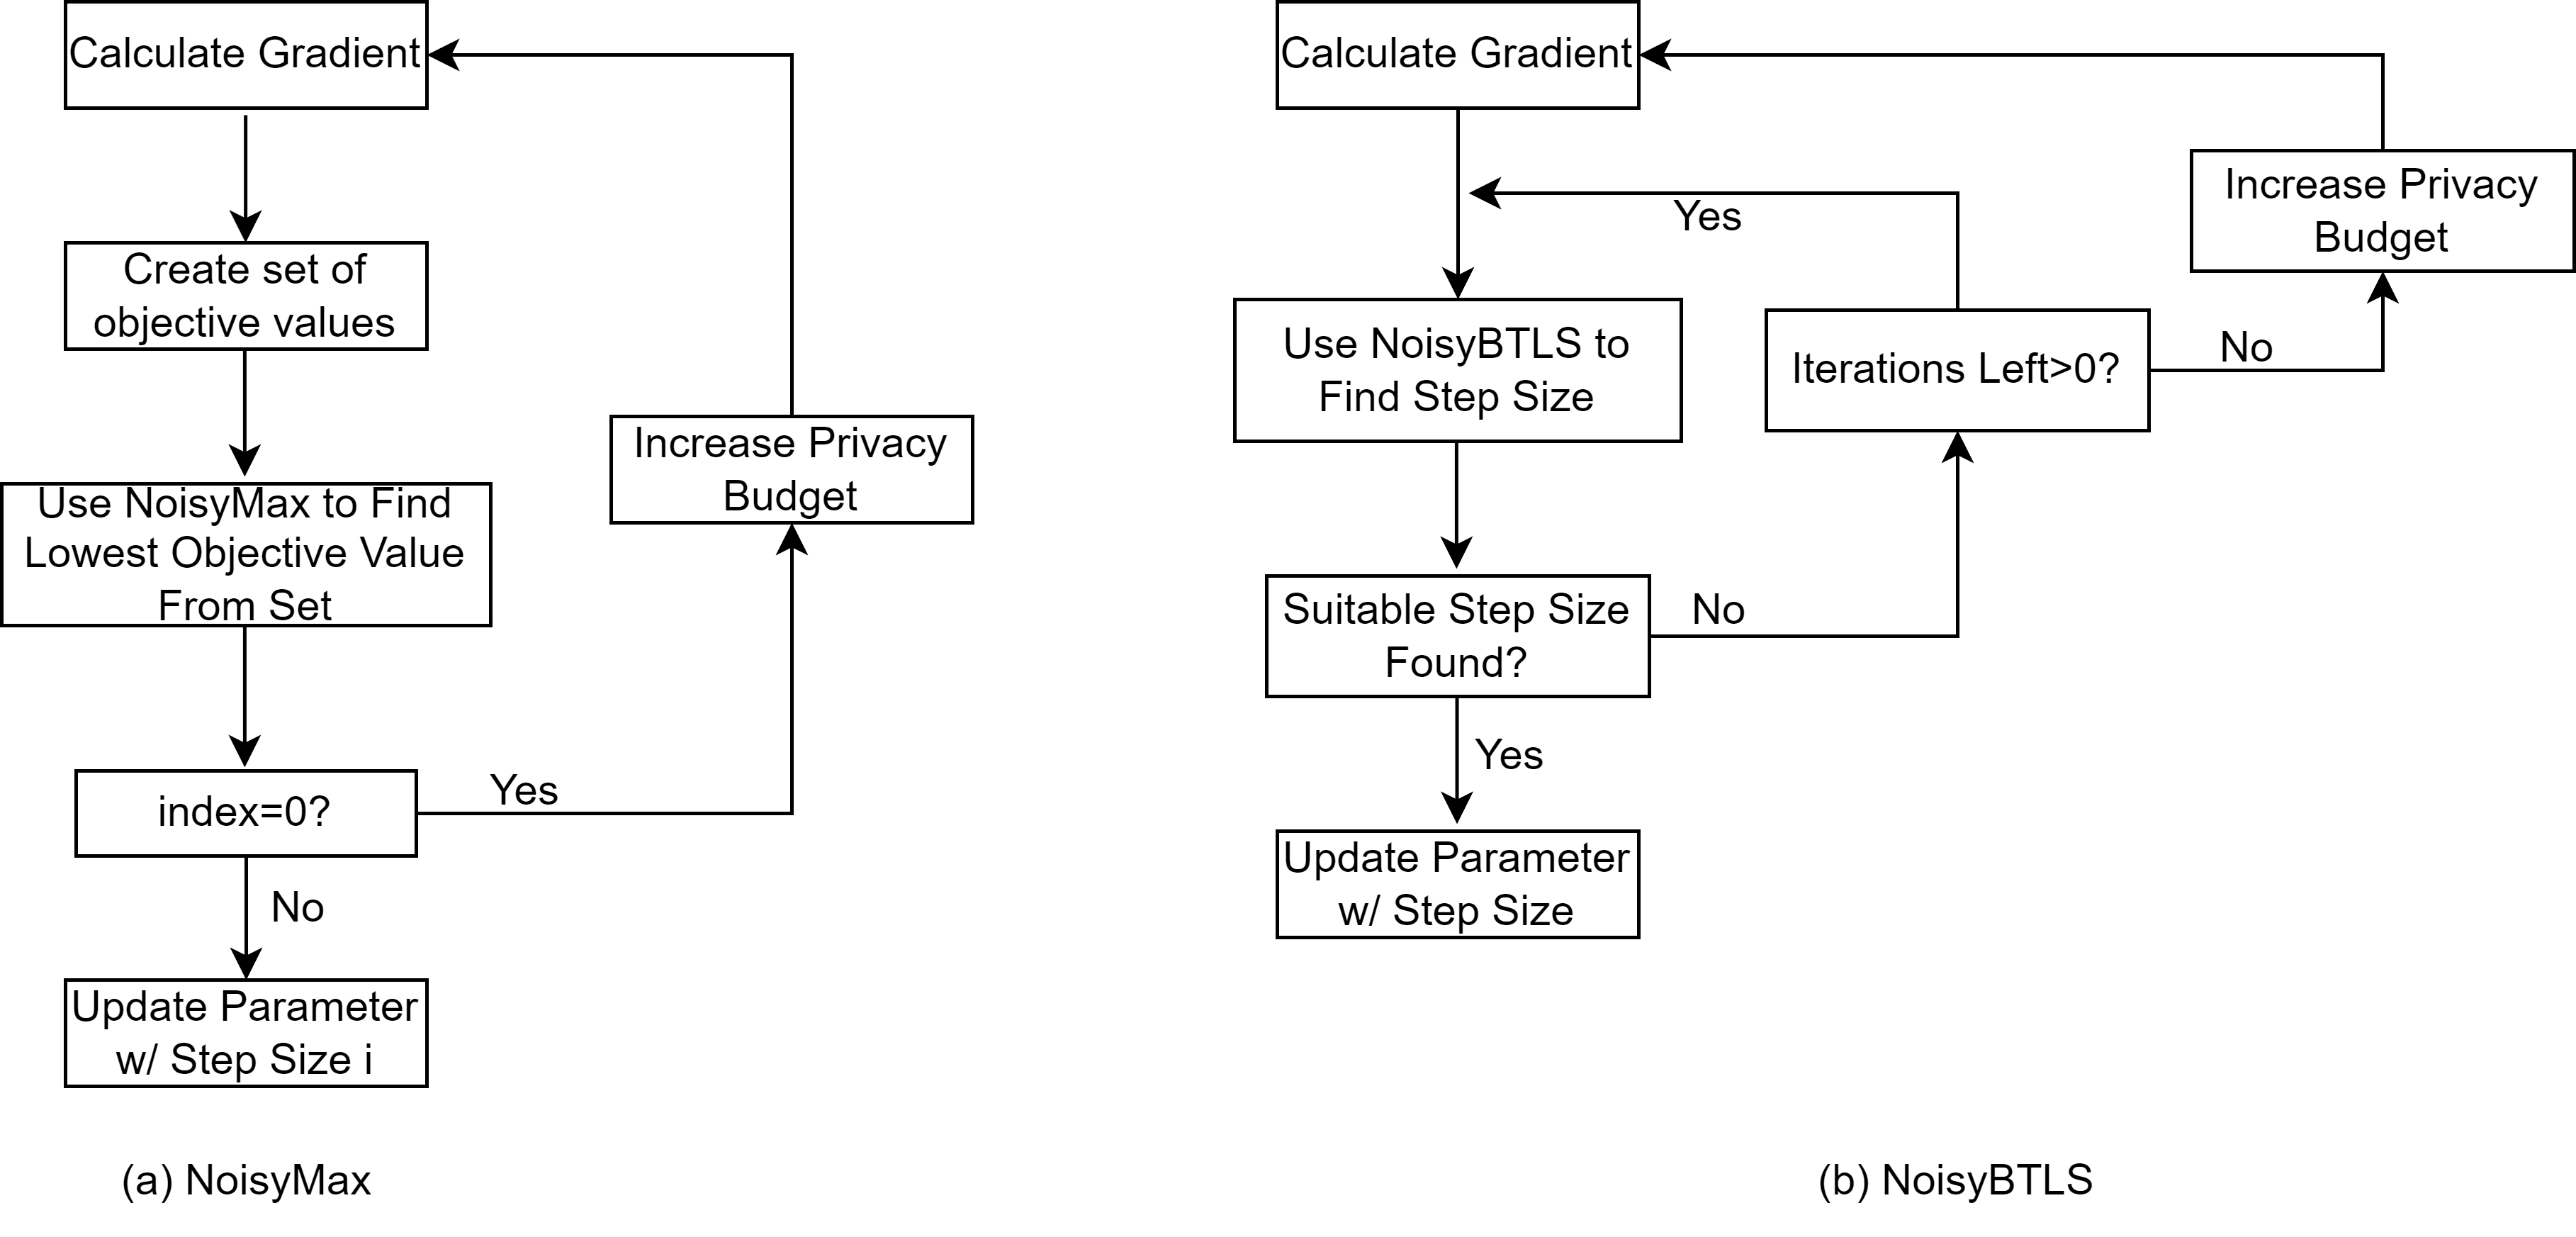
\includegraphics[width=1\linewidth]{submissions/submission5/figs/NoisyMax vs NoisyBTLS2.png}
   \caption{(a) NoisyMax Technique; (b) NoisyBTLS Technique}
   \label{fig:noisymax}
\end{figure} 

As an extension to NoisyMax, the same authors proposed a more advanced approach called Noisy Backtracking Line Search (NoisyBTLS). Similar to NoisyMax, NoisyBTLS adapts both the learning rate and the privacy budget, but in addition it also considers adaptive clipping (which is covered in more detail in Section~\ref{sec:adaclip}).

This method focuses on adapting the learning rate in response to noisy gradient computation while also adjusting the privacy budget using Sparse Vector Technique (also known as the ``above-threshold'' mechanism)~\cite{RefWorks:RefID:61-roth2011interactive,RefWorks:RefID:62-hardtmultiplicative}.
The approach first conducts a backtracking line search in a differentially private manner. %This algorithm is an implementation of the {\em above-threshold} mechanism~\cite{RefWorks:RefID:61-roth2011interactive,RefWorks:RefID:62-hardtmultiplicative}, also known as the {\em Sparse Vector Technique (SVT)}, for the task of line search. 
Figure~\ref{fig:noisymax}(b) illustrates this approach. The algorithm starts by introducing noise to the threshold \( T=0 \), resulting in a noisy threshold \( T=\lambda \), where \( \lambda \) is randomly drawn from a Laplace distribution or alternatively, a Gaussian distribution. Next, multiple iterations are performed, and in each one the following queries are evaluated:

\[ q(\eta,D)=f(w)-f(w-\eta\nabla f(w))-\alpha\eta\|\nabla f(w)\|^2 \]

with added noise \( \nu \) at each iteration. The result is compared with the noisy threshold \( T \). If \( q(\eta,D)+\nu\geq T \), the algorithm outputs \( \eta \) and halts; otherwise, it reduces the step size \( \eta \) by multiplying it with \( \beta \) and continues to the next iteration, where \( \beta\in(0,1) \) controls the rate of step size reduction. This process repeats for a maximum number of iterations. If no limit is set, depending on the noise used in the query, the iteration could lead to an infinite loop or provide minuscule step sizes, which could end up increasing the objective function due to a lack of progress. When the maximum number of iterations is reached, it statistically calculates whether a higher privacy budget is needed, which it then adjusts depending on the results. Due to the use of SVT, the privacy budget needed to find $\eta$ is greatly reduced.

When NOISYBTLS fails to find a step size within the set maximum iteration count, it can lead to two possibilities. The first one is that the current privacy budget $p_{grad}$ is set too small, and the noise dominates the gradient -- Case (1) in the diagram. In this case, the privacy budget needs to be increased. The second possibility is that the noise used in NOISYBTLS is too large and it can’t identify a step size with the right conditions -- Case (2) in the diagram. The remedy to this problem is to increase the privacy budget in order to compute a more precise gradient. To identify which of these two cases are applicable,  the algorithm maintains the moving average of angles between two consecutive gradient values, which gets updated at every iteration:

\[ \theta \leftarrow \text{ANGLE BETWEEN}(g_{t},\tilde{g}_{t})\]
\[\theta = \psi\theta + (1 - \psi)\theta_{t-1} \]

where $\psi \in (0,1)$ is a parameter controlling the decay rate of old information. When $\eta=0$ is returned by NOISYBTLS, the algorithm calculates another gradient $\tilde{g}_{t2}$ using the budget of $\rho_{\text{grad}}$ and measures the angle $\theta$ between $\tilde{g}_t$ and $\tilde{g}_{t2}$). The value of $\theta_{t2}$ is then compared with the moving average-based threshold $\theta_\text{max}$, and if it is larger it would increase the privacy budget $\p_\text{grad}$ for calculating the gradient. Meanwhile, if $\theta$ is less than the minimum threshold $\theta_\text{min}$, the search might fail due to insufficient privacy budget $\epsilon_{BT}$ for the NOISYBTLS. The threshold values $\theta_{\text{max}}$ and $\theta_{\text{min}}$ are calculated as follows:
\[ \theta_{\text{max}} = \phi_{\text{max}} \times \theta, \quad \theta_{\text{min}} = \phi_{\text{min}} \times \theta \]
where $\phi_{\text{max}} > 1$ and $0 < \phi_{\text{min}} < 1$ are hyperparameters. Empirically, this budget adaptation strategy is observed to be particularly effective for convex optimization problems.

In addition to adjusting the privacy budget, it was found that a large clipping threshold is not necessary in the later stages of the training process. Knowing this, the clipping threshold $C_\text{grad}$ and $C_\text{obj}$ is adaptively decreased when the algorithm finds it needs to increase the privacy budget $p_\text{grad}$ during a single SGD update. Even if $p_\text{grad}$ is increased multiple times in a single SGD update, the clipping threshold will only be updated once per update. The clipping threshold is updated as follows:
\[ C_{\text{grad}} \leftarrow (1-\zeta)C_{\text{grad}}, \quad C_{\text{obj}} \leftarrow (1-\zeta)C_{\text{grad}} \]
where $\zeta$ is a hyperparameter that determines the rate of decrease. Since the condition is based on privately released information, it does not consume any extra privacy budget.

\subsubsection{Convergence Rate}
%Above mentioned adaptation trials focus on increasing the privacy budget whenever an optimal step-size cannot be determined. 
Another recent approach to adapting the privacy budget consumption relies on convergence rates~\cite{RefWorks:RefID:49-hong2022dynamic}.
To assess the effectiveness of Private Gradient Descent (PGD), this work utilizes the Expected Excess Risk (EER), a common metric for evaluating the convergence of randomized algorithms. Given the presence of noise and the constraint on learning iterations, optimization using private gradients is expected to lead to a higher loss (excess risk) compared to the optimal solution without privacy constraints. Let \( \theta^* \) be the optimal solution obtained after iterating an algorithm  for \( T \) times. EER quantifies the expected utility degradation as:

\[
\text{EER} = \mathbb{E}[f(\theta_{\nu}^{T+1})] - f(\theta^*).
\]

Due to the variety of loss functions and complexity of recursive iterations, a good estimation of EER in the presence of noise is intractable for most functions. Instead, one can study the worst-case scenario, i.e., the upper bound of EER, with the goal to minimize the upper bound. For consistency, we refer to the upper bound of EER divided by the initial error as \( ERUB \). Since the analytical form of EER is either intractable or complicated due to the recursive iterations of noise, studying \( ERUB \) is a convenient and tractable alternative. The upper bound often has convenient functional forms which are (1) sufficiently simple, so that they can be directly minimized, and (2) closely related to the landscape of the objective depending on both the training dataset and the loss function. As a consequence, it was used in previous literature for choosing hyperparameters. Denote by \( ERUB_{\text{min}} \) the achievable optimal upper bound by a specific choice of parameters, e.g., noise magnitude \( \sigma \) and \( T \).

One can define the influence of noise magnitude \( \sigma \) on EER as the derivative:

\[
q_t^* = \frac{\partial \text{EER}}{\partial \sigma_t}.
\]

Accordingly, one can approximate the EER shift as \( \Delta \sigma \) when \( \sigma \) increases by \( \Delta \sigma \). However, because the EER is strongly data-dependent, the derived \( q_t^* \) on a given dataset may not generalize to another dataset. Instead, one can consider a more general term based on \( ERUB \), i.e., \( q_t^* = \frac{\partial}{\partial ERUB} \sigma_t \).

The work in~\cite{RefWorks:RefID:49-hong2022dynamic} considers the class of loss functions satisfying the Polyak-Lojasiewicz (PL) condition, which bounds losses by their corresponding gradient norms. It is more general than the \( m \)-strongly convexity condition~\cite{RefWorks:RefID:63-polyak1963gradient}. If \( f \) is differentiable and \( M \)-smooth, then \( m \)-strongly convexity implies the PL condition.

The related method in~\cite{RefWorks:RefID:48-fay2023adaptive}  introduces a conceptual framework aimed at dynamically adjusting hyperparameters over time by optimizing the privacy-utility ratio (PUR) at each step. This involves selecting the step size $\eta$ and noise standard deviation $\sigma$ to minimize the privacy loss per unit of utility improvement. The PUR is defined as the ratio of the privacy cost to the utility gain, with utility incorporating convergence metrics like the gradient norm or objective value. Minimizing the PUR enables adaptation of the privacy budget based on optimization progress, with higher precision typically required in later stages as the gradient norm diminishes near the optimum.

Two selection strategies emerge:


\textbf{1. Data-dependent selection:}
   By assuming $F$ is $M$-smooth, a descent lemma estimates the expected improvement in the objective function given step-size and noise variance. Using this lower bound as utility function, along with the privacy cost, one determines hyperparameters that minimize the privacy-utility ratio. Specifically, the privacy-utility ratio is minimized by setting the noise standard deviation $\sigma_t$ proportional to the gradient norm and the step size $\eta_t$ as a constant, given by:
   
   \[ \sigma_t = \frac{\| \nabla F(\theta_t) \|}{\sqrt{d}} \]
   \[ \eta_t = \frac{1}{2M} \]


\textbf{2. Data-independent selection:}  
   A data-independent schedule can be derived based on the PUR-optimal schedule, which is proportional to the gradient norm. This schedule exhibits similar convergence rates to non-private gradient descent (GD), leveraging upper bounds on gradient norms as a proxy for the gradient norm itself.
   
\subsection{Gradient Clipping Adaptation}
\label{sec:adaclip}

The clipping threshold parameter is used to bound the sensitivity of each gradient. A low clipping parameter can result in information being destroyed, and may change the direction of the gradient step. Meanwhile, a high clipping bound increases the sensitivity of training and requires more noise to be added~\cite{RefWorks:RefID:40-abadi2016deep}. It is difficult to achieve a good fixed clipping parameter setting without looking at the training data. Furthermore, weight layers and bias layers need completely different clipping values to be optimal. To tackle this issue, several approaches proposed their own implementation of adaptive clipping. 
%From section 3, we can see how adaptive clipping can provide improvements to the model utility compared to a fixed clipping threshold, and 
In Section~\ref{sec:step} we briefly discussed one method that pairs adaptive clipping with other adaptive parameters. One important aspect is that in a private setup, using gradient norms for tuning requires them to be sanitized first, which means that a portion of the privacy budget must be allocated in each step to protect the norms~\cite{RefWorks:RefID:39-he2022exploring}.

\subsubsection{Norm-based Adaptive Clipping}
\label{sec:normclip}
One of the first proposals of adaptive clipping was introduced by Van der Veen et.al.~\cite{RefWorks:RefID:36-lennarttools} who recognized that choosing a good clipping threshold $C$ is difficult, especially when dealing with multiple layers. They proposed that the clipping bound in the current batch be directly proportional to the $l_2$-norm of the previous batch by a constant factor $\alpha$. This can be summarized in the equation below: 

\[ C_t^l = \alpha|L|^{-1}(\sum_{i\in L_t}\text{clip}(||g_{t-1}^l(x_i)||_2)+\mathcal{N}(0,\sigma_{l^2}^2 C_{l^2t}^l ^2)\]
\[ \text{clip}(||y||_2)=||y||_2/\text{max}(1,\frac{||y||_2}{C_{l^2t}^l})\]

where $C_t^l$ is the clipping bound of the current round $t$ and layer $l$, $g_{t-1}^l(x_i)$  equates to the individual gradient of that layer in previous rounds and privacy parameters $\sigma_{l_2}$ and ${C_{l^2t}^l}$. To calculate the privacy parameter ${C_{l^2t}^l}$, an adaptive procedure is performed similar to clipping, where they sanitize the $l_2$-norm of the previous iteration, $C_{t-1}^l$, multiplied by a constant $\beta$, hence ${C_{l^2t}^l}=\beta C_{t-1}^l$. In this approach, it is required for the user to manually set the values of $\alpha$, $\beta$, and $\sigma_{l2}$, although it has been shown that changing the values of $\beta$ and $\sigma_{l2}$ does not provide meaningful results when measuring test accuracy. 
%Meanwhile, since the approach is adaptive, it is believed a single value of $\alpha$ can provide good results for all tasks.

\subsubsection{Quantile Estimation Adaptive Clipping}
\label{sec:quantile}
The recent work of He et.~al.~\cite{RefWorks:RefID:39-he2022exploring} explores an adaptive clipping technique that uses a form of quantile estimation in the context of per-layer clipping. A portion of the total privacy budget ($r=1\%$ to 10\% of total budget) is allocated for estimating the target quantile for each layer’s gradient norms. The clipping threshold for each layer $C_1,...,C_K$ is then set to the estimated quantile. The number of gradients clipped in each layer is recorded before each parameter update, and the clipping threshold is then adjusted based on how many individual gradients have been clipped previously. The fraction of clipped gradients needs to be sanitized according to DP, and an additional noise multiplier is used to achieve this goal. This also affects the noise multiplier setting for parameter updates, and the new noise multiplier is calculated as:
\[ \sigma_\text{new}=(\sigma^{-2}-K(2\sigma_b)^2)^{-1/2}\]
where $\sigma_b$ is the additional noise multiplier for the sanitized clipped gradients fraction, $\sigma$ is the original noise multiplier and $K$ is the number of layers in the neural network (also known as number of groups).

%The original Gaussian mechanism adds noise right before the release, meaning different coordinates uses the same amount of noise. However, 
The technique also uses different levels of noise in each layer. For example, let $\gamma_1,...,\gamma_k$ be coefficients for scaling, and $\Tilde{g}_k$ be the sum of clipped gradients for layer/group $k$. Applying the Gaussian mechanism to scaled $\hat{g}:= (\hat{g}_1,...,\hat{g}_k)$, where $\hat{g}_k:=\Tilde{g}_k/\gamma_k$, and rescaling back the sanitized values afterwards adds noise to $\Tilde{g}_k$ with standard deviation proportional to $\gamma_k$. There are two ways to choose $(\gamma_1,...,\gamma_K$):
\begin{itemize}
\item Global strategy: $\gamma_k=1$ for $k \in [K]$. This strategy adds same amount of noise to all components.
\item Equal budget strategy: $\gamma_k = C_k$ for $k \in [K]$. This strategy gives all the groups the same privacy budget.
\end{itemize}


Another method of adaptive gradient clipping has been explored in~\cite{RefWorks:RefID:37-andrewdifferentially}, this time in the context of federated learning (FL). %The main contribution to their approach is that proposed method uses negligible amount of privacy budget, and is also compatible with other FL technologies such as compression and secure aggregation. 
The main idea of the approach is to fix the quantile value of observed norms, and use gradient descent to fit $C$ to this value:
\[ \text{Let $X \in \mathbb{R}$ be a random variable, and let $\gamma \in [0,1]$ be a quantile to be matched. For any $C$, define}\] 
\[ l_\gamma (C,X)= 
\begin{cases}
    (1-\gamma)(C-X),& \text{if } X\leq C\\
    \gamma(X-C),              & \text{otherwise}
\end{cases}\]
which implies
\[
\nabla l'_y(C,X)=
\begin{cases}
    (1-\gamma)(C-X),& \text{if } X\leq C\\
    -\gamma,              & \text{otherwise}
\end{cases}
\] 
Since the loss is minimum when $Pr(X<C)=\gamma$, the loss function is convex and gradients are bounded by $1$, it is possible to get an online estimate of $C$ that converges to the $\gamma^\text{th}$ quantile of $X$ using online gradient descent. On a sample size $m$, with $b$ being the proportions of elements lower than $C$, the average derivative of the loss for that round can be simplified to $\Bar{b}-\gamma$. This is captured by the following equation:
\[ \Bar{l'}_\gamma (C;X)= \frac{1}{m}\sum_{i-1}^m
\begin{cases}
    (1-\gamma),& \text{if } x_i\leq C\\
    -\gamma,              & \text{otherwise}
\end{cases}\]
\[ =\frac{1}{m}((1-\gamma)\sum_{i\in [m]} \mathbf{I}_{x_i}\leq c-\gamma \sum_{i\in [m]} \mathbf{I}_{x_i}>c)=\Bar{b}-\gamma\] 
For a particular learning rate $\eta c$, the clipping bound can be updated through: $C\leftarrow C-\eta c(\Bar{b}-\gamma)$. Since $b$ and $\gamma$ take values in [0,1] the update clipping bound changes by at most $\eta \times c$ in each step. This can be a problem in two scenarios, one if $C$ is very large, and the other when updates are coarse and may overshoot to become negative if $C$ is a lot smaller than $\eta c$. The following geometric update rule can be used in this case: $C\leftarrow C \cdot \text{exp}(-\eta c(\Bar{b}-\gamma))$, which allows the update rule to quickly converge to the true quantile even if initial estimates are largely different. Figure ~\ref{AdaptiveClipping} illustrates the adaptive clipping algorithm using quantiles.

\begin{figure}[h]
\centering
    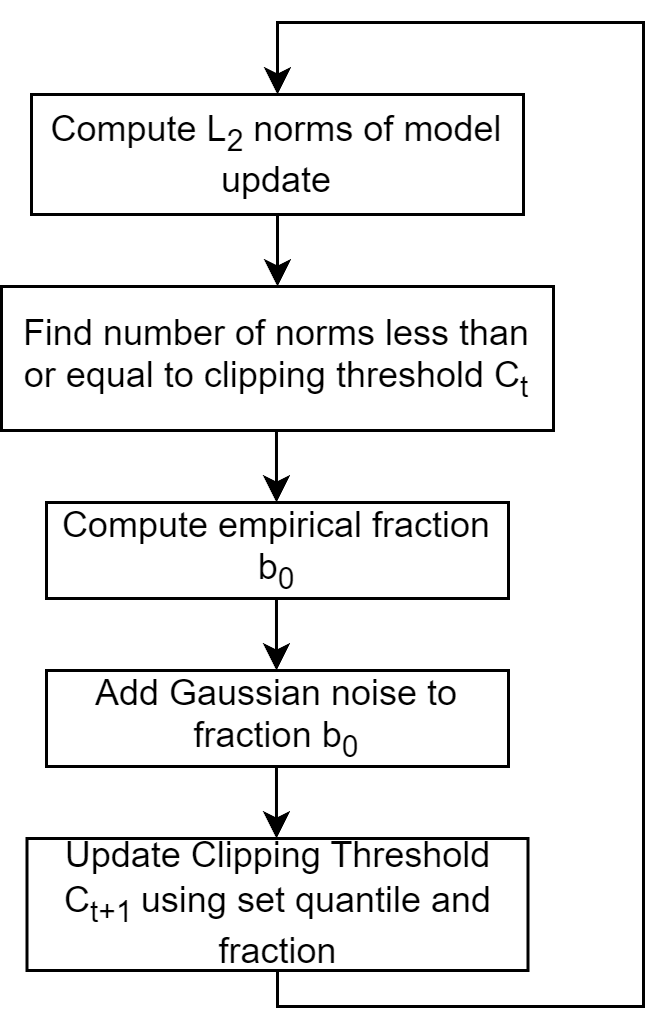
\includegraphics[width=0.3\linewidth]{submissions/submission5/figs/Quantile Estimation.png}
   \caption{Adaptive Clipping Using Quantiles}\label{FigDiff}
   \label{AdaptiveClipping}
\end{figure} 

\subsubsection{Coordinate-wise Adaptive Clipping}
The work of Pichapati et. al.\cite{RefWorks:RefID:35-pichapati2019adaclip:} proposed another approach to adaptive clipping. The {\em AdaClip} algorithm adds less noise compared to other methods by using {\em coordinate-wise} adaptive clipping of the gradient, as opposed to norm-based, thus producing models with improved accuracy. The main idea in the approach is rather than searching for a good clipping value, the gradients are centered and standardized before being clipped to $1$ and then noise is added to their value scaled according to the fixed sensitivity of $1$. The noisy values are then transformed back to their original mean and variance. 

Denote by $g^t$ the stochastic gradient vector at iteration $t$, and let $a^t$ and $b^t$ be auxiliary vectors. The gradient vector $g^t$ is first translated by $a^t$ obtaining $(g^t-a^t)$, then each dimension is divided by $b^t$. This produces the transformed gradient $w^t$, given by $w^t=\frac{g^t-a^t}{b^t}$. Sensitivity is bounded by clipping the transformed gradient at norm 1, according to equation:
\[ \hat{w}^t=\text{clip}(w^t,1)\overset{\Delta}{=}\frac{w^t}{\text{max}(1,||w^t||_2)}\]
Noise is then added to the clipped gradient:
\[ \Tilde{w}^t=\hat{w}^t+N^t\] \[ N^t\sim\mathcal{N}(0,\sigma^2I)\]
Finally, the noisy gradient is rescaled to the same scale as the original gradient by first multiplying with $b^t$ and then adding $a^t$:
\[ \hat{g}^t=b^t\hat{w}^t+a^t\]
This produces the differentially-private approximation of $g^t$. The main challenge consists in finding the optimal choices of the auxiliary vectors $a^t$ and $b^t$. When testing the implementation of AdaClip with the original DP-SGD implementation done by Abadi et al~\cite{RefWorks:RefID:40-abadi2016deep} on the MNIST dataset, AdaClip was found to produce higher accuracy for the same settings of $\varepsilon$ and $\delta$.


\subsection{Learning Rate Adaptation}
\label{sec:lr}
The learning rate parameter controls the step size taken during the optimization process to update the weights of the neural network. Choosing an optimal learning rate is very important: a small learning rate can result in the model taking too long converge, or being stuck at a local optimum. Meanwhile, a learning rate that is too large may result in a model that does not converge. %Typically, the choice of learning rate is done empirically through experimentation and validation, but the introduction of adaptivity allows the learning rate to be adjusted during the training process.

Adapting the learning rate is a concept that has been used in conventional, non-private machine learning, in tasks involving large-batch training~\cite{RefWorks:RefID:53-you2020large}.
%The main goal of adaptive learning rate is updating it depending on the level of trust in each update. Having more confidence in the gradient’s direction means that a larger learning rate can be set. 
In the context of DP-SGD, adapting the learning rate is even more important, as clipping and adding noise to gradients can change the direction of the gradient. %While we have explored solutions that adapted both the privacy budget and the learning rate at the same time in subsection 4.1.2, we will now look into a work that specifically targets learning rate adaptation.
\begin{figure}[h]
\centering
     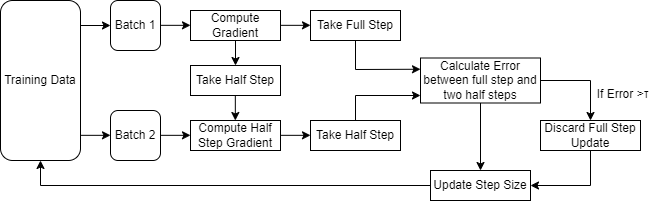
\includegraphics[width=1\linewidth]{submissions/submission5/figs/koskela.png}
   
   \caption{ADADP Update Mechanism}\label{FigDiff}
   \label{fig:koskela}
\end{figure} 

The most prominent approach using adaptive learning rate in private learning has been proposed in~\cite{RefWorks:RefID:38-koskelalearning} by Koskela et al. They proposed a method of adapting the learning rate by estimating the error against the gradient flow when comparing the results after one step and two half-steps. Figure~\ref{fig:koskela} provides an overview of how the algorithm functions, and how the step size is adaptively tuned. The basis of the approach relies on numerical extrapolation of ordinary differential equations (ODEs). Let $g$ be a differentiable function $g:R^d\rightarrow R$. To find the local minimum of function $g$, a first-order method called gradient descent (GD) is used. The gradient flow of $g$ can be described as the explicit Euler method with step size $\eta_l$ applied to a system of ODEs. An estimation of the error of the gradient descent can be performed by considering one step of size $\eta$:
\[ \theta_1=\theta_0-\eta \nabla g(\theta_0)\]
An alternative approach is to employ two steps of size $\frac{\eta}{2}$:
\[ \theta_{1/2}=\theta_0-\frac{\eta}{2}\nabla g(\theta_0) \qquad \hat{\theta}_1=\theta_{1/2}-\frac{\eta}{2}\nablag(\theta_{1/2})\]
It is thus possible to get an $O(\eta^3)$-accurate estimate of the local error through the value $2(\hat{\theta}_1-\theta_1)$. Using this information, the estimation of the error at iteration $l$ can be deduced from $\text{err}_l=||\hat{\theta}_{l+1}-\theta_{l+1}||$. The local error of magnitude $\tau$ to be desired is then set, which is used in the following proposed mechanism to update the step size:
\[ \eta_{l+1}=\text{min}(\text{max}(\frac{\tau}{\text{err}_l},\alpha_\text{min}),\alpha_\text{max})\cdot\eta_l \qquad \label{eq:koskela}\]
where the value of $\alpha_\text{min}<1$ and $\alpha_\text{max}>1$. 
%In the experiments done by this paper, the $\alpha_\text{min}<1$ was set to 0.9 while $\alpha_\text{max}>1$ was set to 1.1. 
When this mechanism is implemented in a DP-SGD setting, the equation to determine the local error is changed instead to be the estimate of the $\ell_2$-norm of the function $\text{err}(\theta,\hat{\theta})$ as it was found to give better numerical results.
\[ \text{err}(\theta,\hat{\theta})_i = \frac{|\theta_i-\hat{\theta}_i|}{\text{max}(1,|\theta_i|)}\]
The way the adaptive DP algorithm works is that a random batch $B_1$ is first drawn with probability $q=|B|/N$. The gradient $G_1$ is then calculated and clipped by $C$, before being evaluated at $\theta_l$. The algorithm then performs two different steps, one by step size $\eta_l$, $\eta_{l+1}\leftarrow\theta_l-\eta_lG_1$,  and the other by half step size, $\frac{\eta_l}{2}$, $\eta_{l+{1/2}}\leftarrow\theta_l-\frac{\eta_l}{2}G_1$. A second set of batches $B_2$ with probability $q$ is then drawn, gradient calculated and clipped $G_2$. This batch, however, is only being evaluated with the half-step size $\eta_{l+{1/2}}$ performed in the first batch, and another half step is performed, $\hat{\theta}_{l+1}\leftarrow\theta_{l+{1/2}}-\frac{\eta_l}{2}G_2$. The error between the updates done by one step size, $\theta_{l+1}$, and two half step size, $\hat{\theta}_{l+1}$ is then evaluated using $||\text{err}(\theta_{l+1}, \hat{\theta}_{l+1}||$. If the evaluated error is greater than the set tolerance parameter $\tau$, the updated parameter is discarded. Regardless of whether the updated parameter was kept or discarded, the next iteration step-size $\eta_$ is then calculated using equation~\eqref{eq:koskela}. 

One of the main advantages of this algorithm is that its privacy properties are simple to analyze. The complete algorithm can be modeled as $\Tilde{M}$ -- a composite of two different mechanisms: $M_{G_1}(X)$ and $M_{G_2}(X)$. The SGD approximation as well as the additive Gaussian noises are independent of each other, meanwhile, the sampling ratio $q$ is kept the same for both. By keeping parameters $q,\sigma$ and $C$ the same for both mechanism, the composite algorithm is able to run half as many iterations as DP-SGD to get the same privacy for the data.

One of the main difficulties in this implementation is choosing a good tolerance parameter $\tau$ that allows the accumulated additive noise to stay bounded as well as preventing any instabilities caused by the SGD gradient. This can be achieved by setting $\tau$ such that the accumulated DP noise after $T$ iterations is approximately $O(1)$ element-wise.

\subsection{Discussion}
\label{AdapDisc}
We explored several categories of techniques for adapting hyperparameters in DP-SGD, all targeting an improvement in the privacy-accuracy trade-off of learning. Table~\ref{tab: adapTable} provides a synthetic classification of the different methods covered in this section, and  the papers in which they were introduced. 
%Ultimately, the main goal of introducing adaptivity to DP-SGD is to improve the performance of the training process, thus increasing the overall accuracy of the model.
\begin{table}[]\centering
\caption{Summary Of Adaptive DP-SGD Approaches}\label{tab: adapTable}
\begin{tabular}{|c|ccc|}
\hline
\multirow{2}{*}{\textbf{Method}} & \multicolumn{3}{c|}{\textbf{Adaptive Hyperparameters}}                                                         \\ \cline{2-4} 
                                  & \multicolumn{1}{c|}{\textbf{Privacy Budget}} & \multicolumn{1}{c|}{\textbf{Clipping}} & \textbf{Learning Rate} \\ \hline
Noise Decay                       & \multicolumn{1}{c|}{\cite{RefWorks:RefID:47-yu2019differentially}}                        & \multicolumn{1}{c|}{}                  &                        \\ \hline
Optimal Step-Size Search          & \multicolumn{1}{c|}{\cite{concentrated},\cite{chen2020stochastic}}                        & \multicolumn{1}{c|}{}                  &    \cite{concentrated},\cite{chen2020stochastic}                    \\ \hline
Privacy-Based                     & \multicolumn{1}{c|}{}                        & \multicolumn{1}{c|}{\cite{chen2020stochastic}}                  &                        \\ \hline
Convergence Rate                  & \multicolumn{1}{c|}{\cite{RefWorks:RefID:49-hong2022dynamic},\cite{RefWorks:RefID:48-fay2023adaptive}}                        & \multicolumn{1}{c|}{}                  &                        \\ \hline
Norm-Based                        & \multicolumn{1}{c|}{}                        & \multicolumn{1}{c|}{\cite{RefWorks:RefID:36-lennarttools}}                  &                        \\ \hline
Quantile Estimation               & \multicolumn{1}{c|}{}                        & \multicolumn{1}{c|}{\cite{RefWorks:RefID:39-he2022exploring},\cite{RefWorks:RefID:37-andrewdifferentially}}                  &                        \\ \hline
Coordinate-wise                   & \multicolumn{1}{c|}{}                        & \multicolumn{1}{c|}{\cite{RefWorks:RefID:35-pichapati2019adaclip:}}                  &                        \\ \hline
Error Tolerance                   & \multicolumn{1}{c|}{}                        & \multicolumn{1}{c|}{}                  &     \cite{RefWorks:RefID:38-koskelalearning}                   \\ \hline
\end{tabular}
\end{table}

In the category of adapting the privacy budget, the advantage gained is achieved by fine-tuning the injected noise at different stages of learning. In the first few iterations, larger gradients are expected, hence a large privacy budget allocation may not help, but as the parameters approach their optimal values, gradients become smaller and require finer-grained tuning, hence the noise should be reduced~\cite{concentrated}. This aspect is further observed in the noise decay approaches, where a simple budget allocation strategy is able to achieve higher accuracy under fewer epochs compared to a uniform privacy budget~\cite{RefWorks:RefID:47-yu2019differentially}. However, that’s not to say the adaptive privacy budget is a perfect solution. There are usually constraints on where this approach is effective. For example, adapting the privacy budget based on the convergence rate requires making assumptions on the loss function, which is not always possible~\cite{RefWorks:RefID:48-fay2023adaptive}. Furthermore, some methods require a public validation dataset to be utilized, and when one is not available, the alternative approach requires setting some additional parameters, which can be difficult to optimize~\cite{RefWorks:RefID:47-yu2019differentially} and will consume budget otherwise allocated to computing gradients.
%This is not to mention the additional computational overhead required to monitor the gradient and make adjustments during each iteration. 

With adaptive clipping techniques, the main advantage gained is eliminating the need to fine-tune the clipping threshold parameter during training. We discussed earlier in the section the importance of setting a good clipping threshold, especially taking into account the sensitivity of the training process. Adaptive clipping helps balance the privacy-utility trade-off to a reasonable degree. In turn, this improves the stability of the training process, preventing extreme cases such as gradient explosions~\cite{RefWorks:RefID:37-andrewdifferentially}. In some cases, adaptive clipping is necessary to achieve good accuracy results compared to a fixed clipping threshold, as observed with per-layer clipping~\cite{RefWorks:RefID:39-he2022exploring}. It is also important to look at the drawbacks associated with adaptive clipping. Some methods, e.g., quantile estimation, require allocating some privacy budget to perform the necessary calculations~\cite{RefWorks:RefID:37-andrewdifferentially, RefWorks:RefID:39-he2022exploring}. Furthermore, a lot of the techniques used to implement adaptive clipping are dependent on additional hyperparameters in order to work, and depending on the sensitivity of these hyper-parameters the algorithm can influence the performance of adaptive clipping~\cite{RefWorks:RefID:35-pichapati2019adaclip:}. It is very difficult to choose an optimal value that can provide the best performance for each method.

The last adaptive hyperparameter we discussed is learning rate. The main advantage seen in adaptive learning rate is accelerating the convergence of the model during the training process. Dynamically adjusting the learning rate based on the gradient updates allows the model to make significant progress in a smaller number of iterations~\cite{RefWorks:RefID:38-koskelalearning}. This is especially the case during the early stages of training, when large model updates are beneficial as they accelerate convergence. However, it is important to factor in the additional computational overhead needed to adjust the learning rate at each iteration. This can end up causing the training time to significantly increase. Similarly to other adaptive techniques, some methods of adaptive learning rate are dependent on more hyperparameters that need to be carefully tuned for performance~\cite{RefWorks:RefID:38-koskelalearning}. It is also important to note that the performance of adaptive learning rate is highly dependent on the datasets and tasks being performed~\cite{concentrated}.

%Overall, introducing adaptive hyperparameters can be a great addition when looking for a boost in accuracy. It is important to consider which methods is most applicable to be used depending on the task that is being accomplished. One common drawback amongst all the adaptive hyperparameters is the need for additional hyperparameters. However, these papers often provides the optimal values needed to be set for each one. This may not be universally applicable depending on the dataset being worked on or the task being performed, but once these hyperparameters are tuned correctly an increase in accuracy and performance and sure to be gained.



\section{Data Management Solutions for DP-SGD}
\label{sec:mgmt}
Memory management has always been a critical challenge in machine learning, particularly in the context of private training. A significant part of the difficulty arises from the model itself, especially with the increasing popularity of Large Language Models (LLMs), which can involve billions to trillions of parameters \cite{RefWorks:RefID:54-rajbhandari2020zero:}. The use of graphics processing units (GPUs) has become popular for training due to their parallel processing capabilities, high throughput, and specialized hardware optimized for matrix calculations, which plays a pivotal role in machine learning during the forward pass and backpropagation process. Despite these computational advantages, leveraging GPUs to their full potential often presents substantial challenges.

Key issues include the limited memory capacity of GPUs, which restricts the size of models and batches that can be processed~\cite{RefWorks:RefID:59-pleissmemory-efficient}. Efficient memory partitioning is necessary to avoid fragmentation and out-of-memory errors but becomes more complex with the additional requirements of DP-SGD, such as gradient clipping and noise addition \cite{RefWorks:RefID:40-abadi2016deep}. Data transfer overheads between CPU memory and GPU memory also pose significant challenges, exacerbated by the frequent updates needed for privacy-preserving operations. Additionally, while multi-GPU training can alleviate some memory constraints, it introduces new complexities in synchronizing gradients and privacy budgets across multiple GPUs.

Understanding and addressing these memory constraints is essential for optimizing the performance and scalability of machine learning models, especially when implementing privacy-preserving algorithms like DP-SGD. A significant challenge in memory management is handling the gradients. Since DP-SGD requires manipulating gradients through clipping and noise addition to preserve privacy, it can significantly influence the memory requirements for training. This section will explore different clipping techniques used in DP-SGD, discussing their key processes and how they impact the memory requirements of training.
\subsection{Flat Clipping}

\subsubsection{Per-example Processing}

One significant drawback of DP-SGD is its perceived computational expense, mainly due to the process of clipping per-example gradients. This process, along with the potential normalization of these gradients, imposes substantial memory and time costs within standard machine learning frameworks~\cite{RefWorks:RefID:56-paszke2019pytorch:}. As a result, private machine learning techniques like DP-SGD become even more computationally and memory intensive compared to their non-private counterparts~\cite{RefWorks:RefID:43-dupuy2022efficient}.

The computational and memory cost of training depends on the technique being used in taking the training data before performing the private training that would effect how the dataset gets clipped in each iteration. The most basic one is per-example clipping, where only one example from the dataset is used in each iteration of the training. Since only one example is being processed at any given time, this can end up easing the memory requirement of the training process. However, it may still be prone to issues in terms of memory management. In particular, these issues can arise from having a large model with billions of parameters, in which the advantage of only processing one example at a time becomes negligible in terms of memory space. In such cases, a solution would be to partition the model into different memory segments, or assign each partition to different GPU units~\cite{RefWorks:RefID:60-lv2023full}. In the latter case, the overhead introduced in communicating and synchronizing the different GPUs would also need to be considered. Furthermore, this issue can also arise when working with a model that contains multiple layers. The aggregation of the gradient from these layers can end up not fitting in a memory, necessitating to partition the gradients between different memory blocks. Since this issue mainly stems from needing to store the per-example gradient in order to calculate the norm needed for clipping, alternative approaches to clipping can be introduced which do not rely on the gradient norm. This would solve the overall need of storing the per-example gradient in memory. However, it is important to note that per-example clipping tends to require the least memory compared to other clipping techniques as only one example is being worked on at a time. The downside consists mainly in its computational inefficiency, as more iterations are required to go through enough of the training data, and difficulty of implementing parallelism in this method wastes some of the hardware utilization potential.

\subsubsection{Minibatch Clipping}

Mini-batching processes a subset of examples from the dataset (a minibatch) at the same time for each iteration. Compared to per-example clipping, minibatching has the advantage of being more computationally efficient, as less iterations are needed to process the same number of examples. Hardware utilization is also more efficient due to allowing parallelization and vectorized operations~\cite{RefWorks:RefID:55-leescaling}. However, it is widely acknowledged that minibatch clipping will require more memory usage compared to other techniques. Not only do all the examples need to be stored, but the related activation function result and gradient would end up needing to be stored to perform the clipping. As seen for per-example clipping, if the model itself ends up taking a large amount of memory space, this problem would be exorbitantly worse in the minibatch setting. The overall memory size requirement can be dictated by the batch size multiplied by the size of each example in the batch, meaning the bigger the batch size, the more memory is required \cite{RefWorks:RefID:51-yousefpouropacus:}.  Additional temporary memory buffers must be allocated for the aggregation of the gradients in the minibatch before noise can be added and the parameters can be properly updated. However, if small batches are used to reduce memory overhead, it would result in lower computational performance as it limits the capabilities of parallelization~\cite{RefWorks:RefID:58-shirish2017large-batch}.

To ease the memory requirement, the aggregation of the gradients can be done from the start, eliminating the need to store the per-example gradients of the batch, but realistically this is applicable only for clipping techniques that do not rely on the gradient norm. Alternatively, the idea of gradient accumulation can be implemented to reduce the memory needed~\cite{RefWorks:RefID:46-ponomareva2023dp-fy}. The concept works similarly to microbatching, which is explained later. Similar to previous steps, a small batch is taken and the gradients in the batch are clipped and aggregated into one memory block. The next batch is then drawn and gradients of the batch are clipped again, but this time instead of storing them separately from the first batch, they would all be accumulated in one running sum. This repeats for a number of steps before performing the gradient step with noise addition to do the parameter updates. This technique allows for an arbitrarily large batch while requiring a fixed amount of memory.

\subsubsection{Microbatch Clipping}
Microbatching takes mini-batching further, by dividing the minibatches to even smaller sub-batches called micro-batches. This technique eases up the memory requirements of minibatching, by working with fewer inputs at any given time. Assume a minibatch with a size of 32, meaning that 32 activations and gradients need to be stored simultaneously. Assume we introduce microbatching and split the minibatches into 4 microbatches of size 8 each, we would then only need to hold 8 instances of activation and gradients at the same time. Once the current microbatch has finished, only the final aggregated gradient of the microbatch needs to be stored, and the memory to store the previous gradients would then be used for the next iteration. These microbatch gradients would all be accumulated in one memory block that stores the overall aggregated gradient of the microbatch. Figure~\ref{minibatchvsmicrobatch} shows a comparison between the differences of minibatch clipping and microbatch clipping. One of the main advantages is the ability to add noise to each micro-batch as opposed to the aggregated gradient in mini-batching, allowing tighter control over the DP mechanism and allowing more precise tuning to the privacy required~\cite{RefWorks:RefID:46-ponomareva2023dp-fy}. However, this additional noise can also result in reduction in the model's utility. Microbatching also results in higher runtime compared to traditional minibatching, as it limits the capabilities of the hardware utilization compared to traditional minibatching due to the need to process the micro-batch sequentially~\cite{RefWorks:RefID:51-yousefpouropacus:}. It may seem counter-intuitive to use microbatching, given that minibatching offers greater computational advantage and there is the option to simply reduce the batch size to handle the memory problem, but in some cases microbatching is the only alternative solution that is available. For example, a single GPU may not be sufficient to support large batch sizes. By utilizing micro batching, the peak memory required is significantly reduced, allowing the handling of larger batch sizes with limited resources~\cite{databricksFarewellCUDA}.
\begin{figure}[h]
\centering
        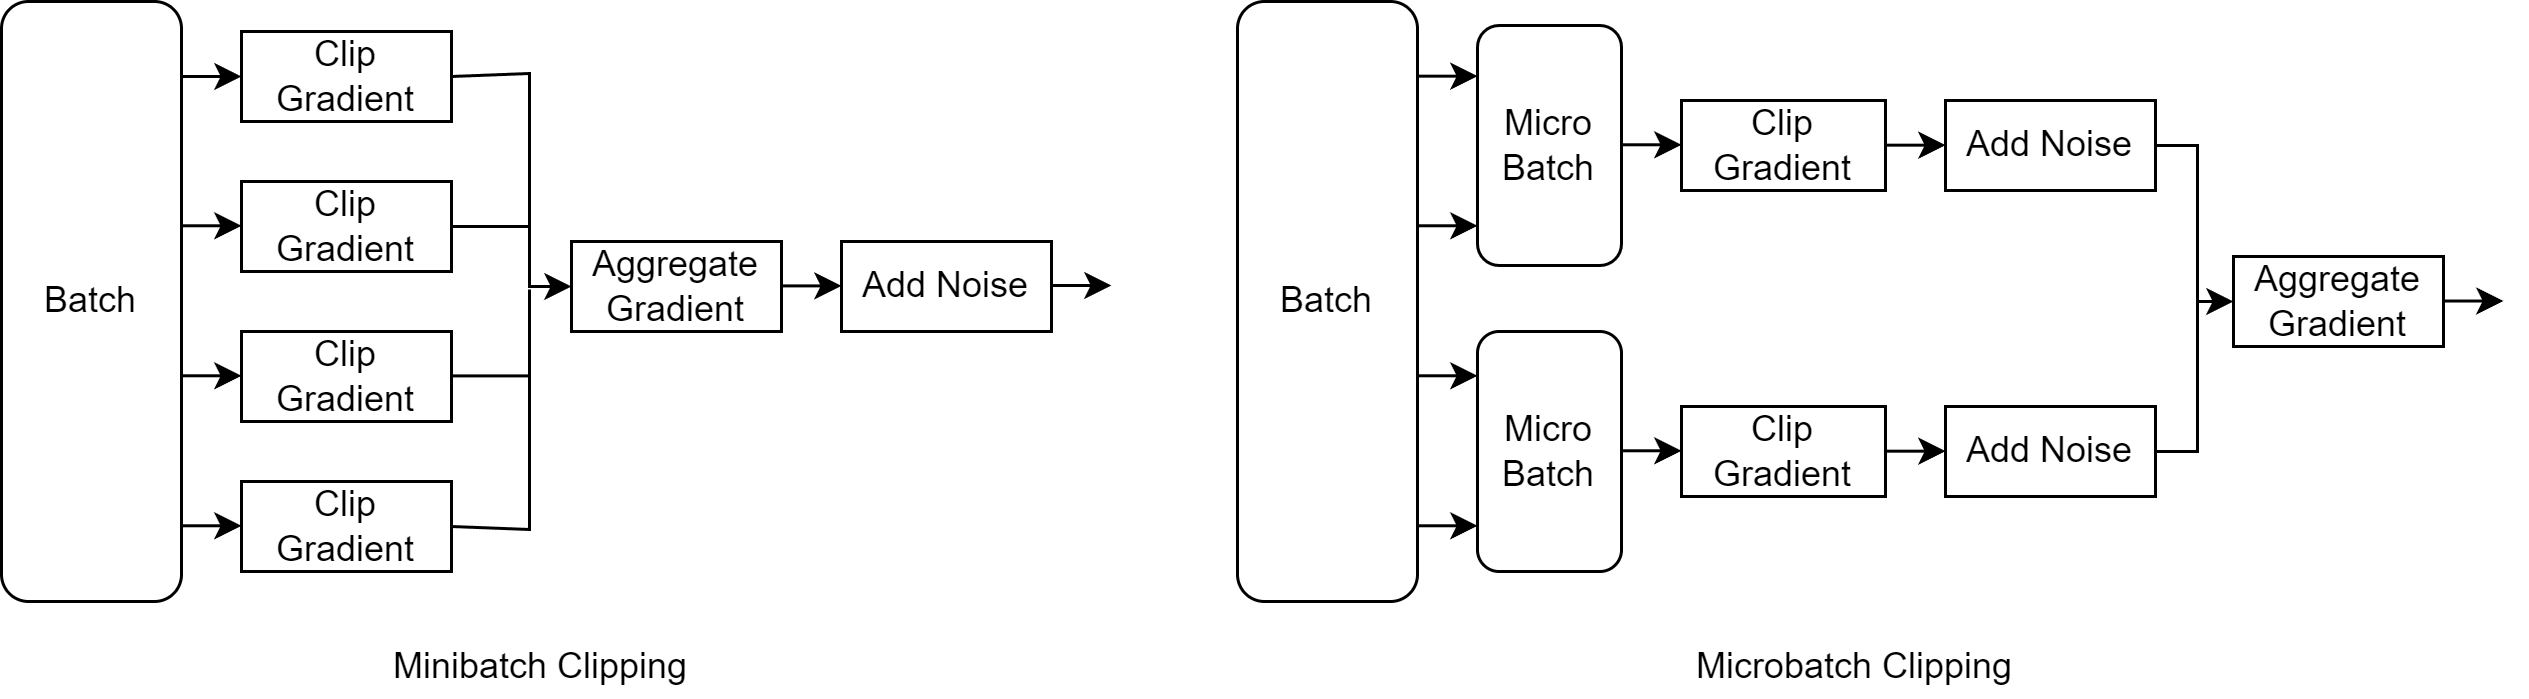
\includegraphics[width=1\linewidth]{submissions/submission5/figs/mini vs micro.png}

   
   \caption{Minibatch Clipping vs Microbatch Clipping}\label{FigDiff}
   \label{minibatchvsmicrobatch}
\end{figure} 

To combat the high memory and computational demands of DP-SGD, several works investigated solutions that ease the cost of DP-SGD, especially in the contest of large-scale models.  McMahan et al.~\cite{RefWorks:RefID:45-mcmahan2018learning} modified federated learning techniques for DP-SGD and distributed the training process to different mobile devices that share the same model. Dupuy et al.~\cite{RefWorks:RefID:43-dupuy2022efficient} proposed another technique for group-wise clipping involving the use of GPUs. Since DP-SGD is computationally expensive because each batch requires its own gradients, these batches can instead be divided into micro-batches and assigned their own GPU. This reduces the computational cost of computing the overall gradient as the work is divided between the GPUs. %Furthermore, scaling and noise addition is done independently by each micro-batch, where once each micro-batch finishes its computation, their clipped noisy gradient and the model aggregates all of the to return an overall gradient. 


\subsection{Group-wise Clipping}

%Although these techniques offers valuable solutions for large-scale training, the focus on these papers are not on improving the efficiency of DP-SGD. Author 
He et al.~\cite{RefWorks:RefID:39-he2022exploring} investigated group-wise clipping for its memory and processing advantage compared to traditional flat clipping, regardless of the size of the model. Two group-wise clipping techniques were considered: per-layer clipping and per-device clipping.

\subsubsection{Per-layer Clipping}
\begin{figure}[h]
\centering
         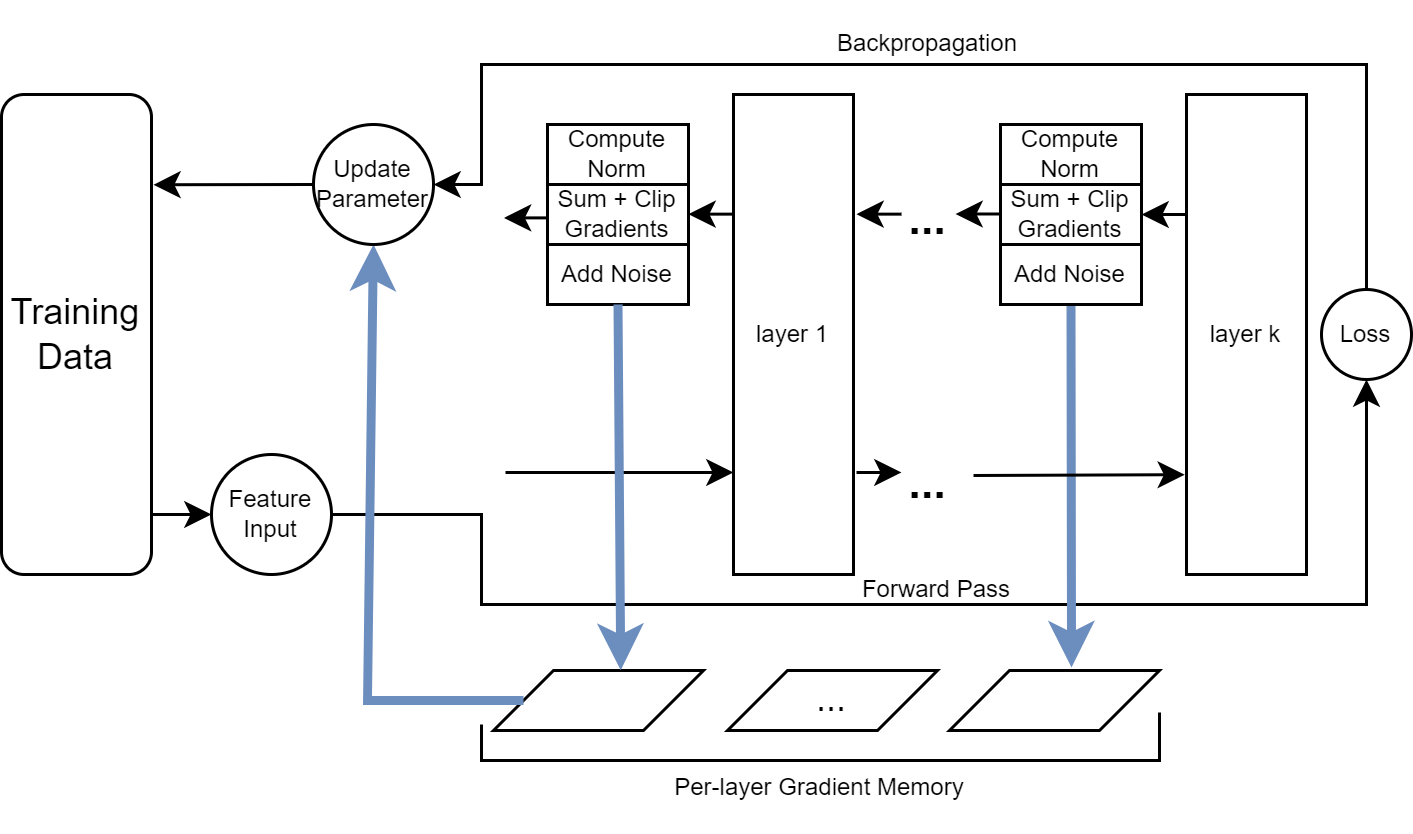
\includegraphics[width=1\linewidth]{submissions/submission5/figs/Per Layer Clipping.png}      
   \caption{Per-layer Clipping}\label{FigDiff}
   \label{perlayerclipping}
\end{figure} 
In per-layer clipping, per-example gradients of each layer in a neural network are clipped separately. Parameters of a neural network are grouped together and each of the $K$ layers in the network is prescribed its own clipping threshold, $C_k$. This brings the main advantage of per-layer clipping, in which gradient clipping for a particular layer can be done as soon as the backpropagation returns the output gradient of that layer, allowing clipping to be done together with backpropagation, as opposed to flat clipping which requires backpropagation to completely finish first. Additionally, the process of summing and clipping of the per-example gradient can be combined as soon as the input activation, output gradients and per-example gradient norms are known. Figure~\ref{perlayerclipping} shows the entire training cycle and how each layer performs its gradient computation, as well as how each layer's gradients are stored separately to perform the parameter updates corresponding to each individual layer. Besides the computational advantage, this method does not require instantiating the per-example gradients in memory, and instead can be computed as needed. This technique is referred to as ghost clipping~\cite{RefWorks:RefID:44-li2022large}. 
%The extra computations for the gradient norm and scaling are often cheap, making this method of private training not just memory-efficient but also time-efficient compared to the non-private counterpart for small to moderate scale workflow.

However, even though a computational advantage is noticed for per-layer clipping, utilizing a fixed clipping threshold for each layer ends up making the model perform worse compared to the traditional flat clipping method in certain scenarios. Observations during training reveal significant fluctuations in the magnitudes of per-layer gradients throughout the process. While gradients may initially be uniformly low, they tend to increase notably for layers closer to the input as training progresses. It is suggested that employing a fixed layer-wise clipping threshold eliminates the structural relationship between gradients of different layers, introducing an additional source of bias on top of the inherent bias associated with flat clipping techniques. As a solution to the performance problems of fixed per-layer clipping, adaptive clipping thresholds can alleviate the structural bias that comes with clipping gradients of different layers separately. In this case, the adaptive clipping technique focuses a quantile estimation, as discussed in Section~\ref{sec:adaptation}.

\subsubsection{Per-device Clipping}

Another group-wise clipping technique explored in~\cite{RefWorks:RefID:39-he2022exploring} is per-device clipping. The main motivation for this method is to make use of larger/better pre-trained model as past works have shown using them improves the privacy-utility trade off. The problem is that size of the model makes it so that the model weights cannot be fit in a single device (GPU), making it a difficult computational problem. The solution to this problem revolves around pipeline parallelism popularly used in non-private training~\cite{RefWorks:RefID:50-huanggpipe:}. The model is first partitioned into consecutive blocks/layers which is then assigned to its own accelerator (i.e., GPU). Forward computation is performed on micro-batches (split mini-batches) that chain together the local computations done on each model partition by communicating activation outputs between the GPUs. Backpropagation reverses this process but on each GPU, and intermediate forward computations are performed to reduce peak memory usage. Furthermore, parallel computation is enabled across GPUs to reduce overall training time. Once all micro-batches finish their forward and backward computation, SGD performs its parameter updates, and the GPUs are synchronized.

Since flat clipping requires computing per-example gradient norms in order to get the scaling factors for computing gradients, it becomes necessary to have additional communication between devices to get the per-example norms of their local gradients. This ends up adding extra overhead to the pipeline parallelism process~\cite{RefWorks:RefID:39-he2022exploring}. There are three potential approaches to reduce communication, however both of them result in non-trivial slowdowns and increased complexity in the implementation. The first approach is to synchronize all the devices after the full backward pass is finished for each micro-batch. This allows each device to have the same gradient norms for computing the clipping scaling factor, but it ends up requiring as many synchronization steps as the amount of micro-batches in a mini-batch, which further reduces efficiency when micro-batches are large. 
%Although this is executing the primitives themselves are not costly, the disruption caused to the pipeline by the frequent calls ends up becoming costly. The devices ends up needing to perform one of three options; the first is to keep the unclipped local per-example gradients for the micro-batches, and to keep being idle until micro-batch synchronization is called to avoid any memory errors, which is a problem initself as resources are being wasted keeping the devices idle. 
The second option is to offload the unclipped local per-example gradients to the CPU, and to transport them back during synchronization. The problem here is the slow CPU-GPU data transfer rates ends up being costly. The last option is to re-materialize the local per-example gradient during synchronization, which ends up being costly as it requires a second  backpropagation step to be performed. 
%As seen, all the options incurs some kind of performance loss.

%As an alternative, a new per-device clipping scheme is proposed where each device is assigned it's own clipping threshold for clipping the per-example gradients of the hosted model piece. Using the equal budget strategy discussed earlier, the noise level added to the gradients in each device is independent of each other, which means no extra communication is necessary.


\subsection{Quantifying Memory Requirements}
\begin{figure}[h]
\centering
    \subfloat [Per-layer Clipping\label{fig:subfigA}] {
        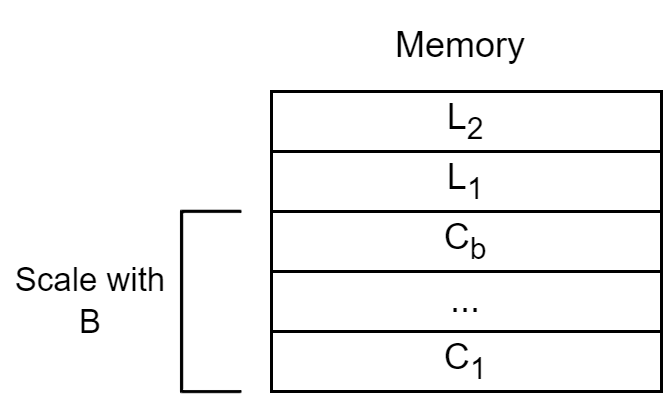
\includegraphics[width=0.4\linewidth]{submissions/submission5/figs/PerLayer.png}}
    \qquad
    \subfloat[Mini-batch Clipping\label{fig:subfigB}]{
          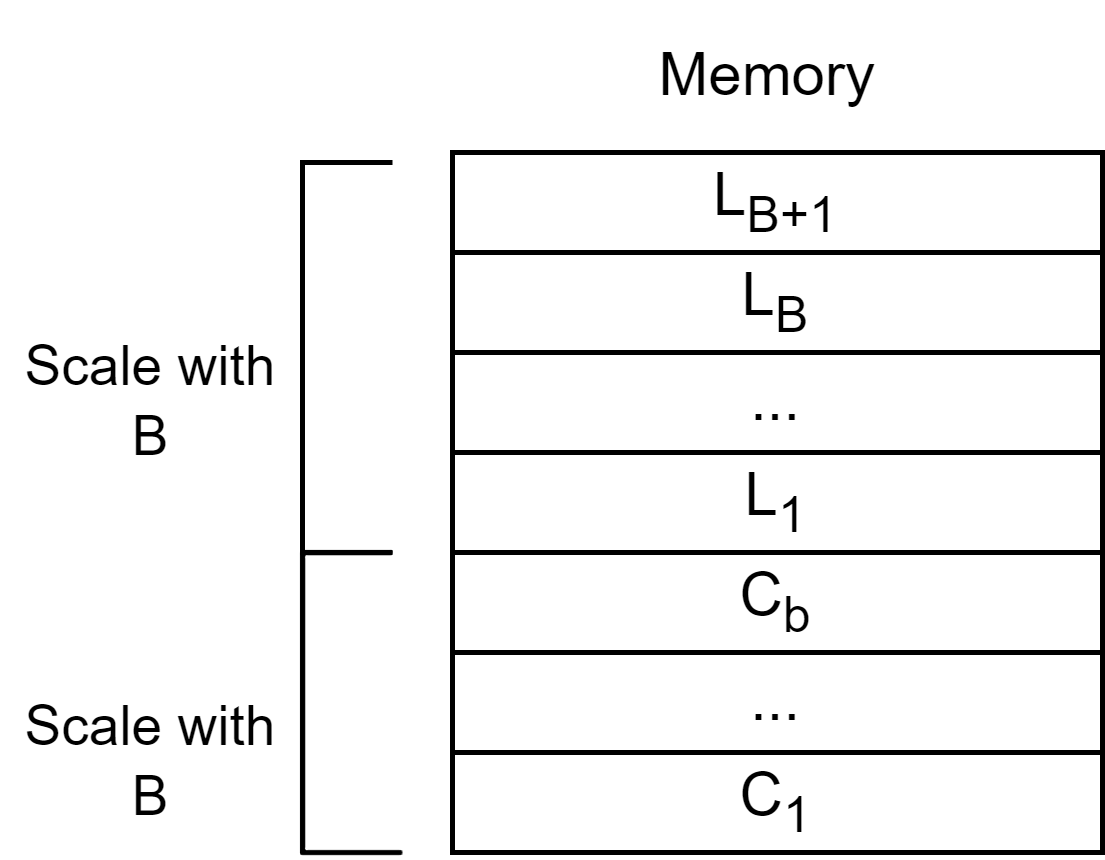
\includegraphics[width=0.4\linewidth]{submissions/submission5/figs/Minibatch.png}}    
   
   \caption{Per-layer Clipping Memory vs Mini-batch Clipping Memory}\label{FigDiff}
   \label{ClippingMemory}
\end{figure} 
Knowing the different ways clipping can be performed, it is important to quantify how much memory is required by each technique. Yousefpour et. al.~\cite{RefWorks:RefID:51-yousefpouropacus:} estimated the memory requirements in a per-example setting that uses the minibatching technique as follows:
\[ \text{M}_\text{non-DP}=bC+2L\]   
\[ \text{M}_\text{DP}=bC+(1+b)L\]
where $L$ is the number of trainable parameters with each one being of size $1$, $C$ is the size of the features, label, and model output for a single data point, and $M$ is the total memory usage for one forward and one backward pass on a batch of size $b$. The labels and outputs for $b$ data points are expected to occupy memory of size $bC$ and the model itself occupies memory of size $L$. In a non-private setting, the gradients are expected to occupy an additional memory of size $L$, meanwhile, for a private setting, the gradients are expected to occupy a memory of size $bL$ due to the need to store per-sample gradients. If the batch size is greater than or equal to 1, it's possible to get an estimate of how much memory private training requires compared to non-private as a ratio of the number of trainable parameters and the size of the model input/outputs. This is given as:
\[
\frac{\text{M}_\text{DP}}{\text{M}_\text{non-DP}} = \begin{cases} 
\frac{bC+(1+b)L}{bC}=1+\frac{L}{C}, & \text{if } L/C<<b \\
\frac{2+b}{3}=\frac{b}{3}, & \text{if } L/C=b \\
\frac{1+b}{2}=\frac{b}{2}, & \text{if } L/C>>b 
\end{cases}
\]


He et. al.~\cite{RefWorks:RefID:39-he2022exploring} compared the memory requirements between the per-layer clipping and the approach in~\cite{RefWorks:RefID:51-yousefpouropacus:} and found that per-layer clipping occupies a similar amount of memory as the non-private setting. This result is expected, given that the ghost clipping technique used in per-layer clipping eliminates the need to store per-sample gradients, making the memory requirement of storing the gradient independent of the batch size. This means that the traditional mini batching technique would require double the memory size compared to per-layer clipping, as traditional mini batching scales with the batch size twice, as opposed to only once with per-layer clipping. Figure~\ref{ClippingMemory} shows a comparison between the scaling factor with the batch size in terms of memory for per-layer clipping and mini-batch clipping. As an example, assume $L$ and $C$ both uses a memory unit of size $1$, and training uses a batch size of $100$. Using the equation above, we can estimate the memory required for traditional mini batch clipping with per-sample gradients to be $201$. Meanwhile, for per-layer clipping, we would need a memory block of size $102$ only. The difference will keep growing bigger with larger batch size, especially when we consider private training of large-scale models that require the use of multiple GPUs.


\section{Individualized Privacy Budget}
\label{sec:individ}

The majority of DP-SGD techniques assume a fixed privacy requirement (i.e., budget $\varepsilon$) for all data contributors, and focus on various adaptations of learning rate or budget consumption throughout the learning process to improve the privacy-accuracy trade-off (see Section~\ref{sec:adaptation}). The privacy budget used in the training must adhere to the most stringent privacy requirement among all data contributors. However, in practice, various data contributors may have differing privacy expectations~\cite{userConc}. Data points from contributors with lower privacy requirements could potentially offer more valuable information for training machine learning models. Consequently, setting a uniform privacy budget across all data points may unnecessarily lower the training accuracy.

Recently~\cite{ipate}, a novel research direction has surfaced, which focuses on supporting the enforcement of heterogeneous privacy constraints across the training dataset. Data points are partitioned into several groups, each with its own privacy budget. Essentially, the concept involves allocating greater privacy budgets to less sensitive data points and lower budgets to more sensitive ones. In this section, we review the several approaches for {\em individualized} privacy budget assignment.

The idea of individualized privacy constraints has been considered in the differential privacy literature even before DP-SGD emerged, in the context of statistical queries. The early work by Jorgensen et. al. \cite{Jorgensen2015} proposed two directions. The first one involves a two-step process: non-uniform sampling based on each tuple's specific privacy requirements, followed by applying a differentially private mechanism to the sampled dataset. This method effectively combines randomness from both steps to achieve personalized privacy guarantees. The second approach, inspired by the exponential mechanism developed by McSherry and Talwar \cite{mcsherry2007mechanism}, offers a more direct route to achieving Personalized Differential Privacy (PDP). 

Later on, the work done by Li et. al. \cite{li2017partitioning} explored two partitioning methods aimed at achieving PDP while optimizing individuals' privacy budgets and enhancing utility. These methods, termed {\em privacy-aware} and {\em utility-based} partitioning, group records with diverse privacy budgets into different bins. Each bin undergoes DP aggregate computation using its minimum privacy budget, and the perturbed results are aggregated in the final output.

A recent study \cite{Niu2021} took an adaptive approach to PDP. The proposed adaptive framework for personalized differential privacy ({\em AdaPDP}) dynamically selects noise generation algorithms and determines parameters such as sensitivity and noise magnitude based on query functions, data distributions, and privacy settings, in order to maximize data utility. Additionally, AdaPDP conducts multiple rounds of utility-aware sampling to meet diverse privacy requirements for individual users.

Most studies emphasize two key directions to achieve individualized privacy: {\em sampling} and {\em grouping}. In the former approach, sampling probabilities are assigned to data points inversely proportional to their privacy concerns, ensuring that records with higher privacy demand are sampled less frequently. In the latter, points with equal privacy concerns are clustered together, with higher-privacy groups undergoing more noise addition than lower concern groups. Figure~\ref{sampleGroup} illustrates the two approaches.

\begin{figure}[h]
\centering
    \subfloat [Sampling\label{fig:subfigA}] {
        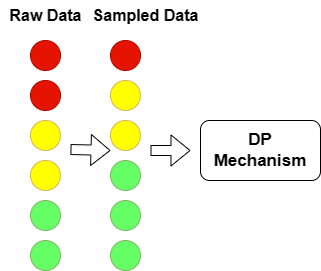
\includegraphics[width=0.4\linewidth]{submissions/submission5/figs/sample.png}}
    \subfloat[Grouping\label{fig:subfigB}]{
          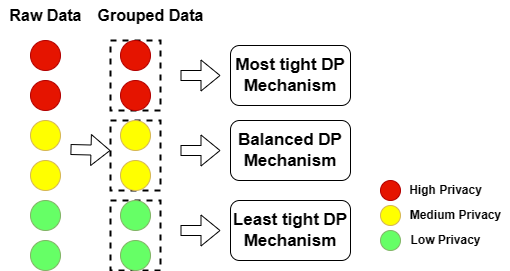
\includegraphics[width=0.6\linewidth]{submissions/submission5/figs/grouped.png}}    
   
   \caption{Sampling Approach vs Grouping Approach}\label{FigDiff}
   \label{sampleGroup}
\end{figure} 

%In the upcoming lines we are going to discuss different approaches that adapted the same concept for the differentially private deep learning.

The \textbf{upsampling} approach is a technique introduced in~\cite{ipate} in conjunction with the Private Aggregation of Teacher Ensembles (PATE) algorithm. PATE is an alternative to DP-SGD for training machine learning models on sensitive data while preserving individual privacy. It involves training multiple teacher models on disjoint subsets of the data, aggregating their predictions with differential privacy, and then training a student model using the noisy aggregated labels. PATE allows for effective model training while ensuring privacy protection, making it suitable for various applications in fields like healthcare and finance~\cite{pate}.

The upsampling mechanism relies on duplicating sensitive data
such that overlapping data-subsets can be allocated to different teachers. Thereby, data with higher privacy budgets are used to train a
higher number of teachers, thus revealing more information from data points with less restrictive privacy needs, and restricting the level of information derived from points with higher demands~\cite{ipate}. The algorithm ensures that points are duplicated by an integer according to the privacy budget ratios. Algorithm~\ref{algo:algPATE} shows how the upsampling factor is calculated for each data point.

\begin{algorithm}[H]
\SetAlgoLined
\KwIn{Privacy budgets $\{ \varepsilon_d \}$ for each data point $d$, precision $p \in \mathbb{N}$}
\KwOut{Upsampling factor $u_d$ for each data point $d$}
{ $\{ \varepsilon_1, \ldots, \varepsilon_j \} \leftarrow \text{unique}(\{ \varepsilon_d \})$ } \tcp*{Get unique budgets}
\For{each $\varepsilon_j$}{
    $\bar{\varepsilon}_j \leftarrow \varepsilon_j \cdot 10^p$ \tcp*{Upscale budgets}
}
$D \leftarrow \text{Greatest Common Divisor}(\bar{\varepsilon}_1, \ldots, \bar{\varepsilon}_G )$; \\
\For{each $\bar{\varepsilon}_j$}{
    $u_d \leftarrow \frac{\bar{\varepsilon}_j}{D}$; \\
}
\caption{Upsampling method in PATE~\cite{ipate}}
\label{algo:algPATE}
\end{algorithm}

Using the same upsampling technique, the work in~\cite{haveit} proposed a method that relies on sampling data points with different sample rates ${q_1, . . . , q_P }$ depending on their individual privacy budgets. In this case, the noise multiplier $\sigma_{sample}$ is fixed. Data points with higher privacy budgets (weaker privacy requirements) are assigned higher sampling rates than those with lower privacy budgets. This modifies the Poisson sampling process for DP-SGD to sample data points with higher privacy budgets within more training iterations.
Using the minimum privacy budget of $\epsilon_1$, the algorithm begins by initializing the $\sigma_{sample}$ with $\sigma$ from conventional DP-SGD, which is the noise multiplier needed for the privacy group $G_1$, which has the strongest privacy requirement of all groups. This is equivalent to instantiating $\sigma_{sample}$ using the overall privacy groups' upper bound noise. Next, they employ a $getSampleRate$ function to determine the sample rates for the specified privacy parameters. The algorithm then reduces $\sigma_{sample}$ repeatedly by a scaling factor that is marginally smaller than $1$, and  recalculates ${q_1,...,q_P}$ until their weighted average approaches $q$ (the traditional unified sampling rate).

The \textbf{grouping} approach is another technique used for individualized privacy budget assignment, which clusters together training examples with similar privacy requirements. In PATE, this step takes the form of a {\em weighting mechanism}~\cite{ipate} which adjusts how the aggregation of teacher votes is performed. It does this by assigning higher or lower weights to individual teachers' votes based on the privacy requirements of their training data points. Consequently, data points with similar privacy budgets $\varepsilon_j$, referred to as a privacy group $g_j$, must be assigned to the same teacher(s). Algorithm~\ref{algo:algPATE2} outlines the process of assigning weights $w_i$ to the teachers.

\begin{algorithm}[H] 
\SetAlgoLined
\KwIn{Privacy budget $\varepsilon_j$ and number of teachers $n_j$ for each privacy group дj, $j \in \{1, \ldots, G\}$, and total number of teachers $k$}
\KwOut{Weight $w_i$ for each teacher $t_i$}
$E \leftarrow \sum_{j=1}^{G} \varepsilon_j$; \\
\For{each privacy group $g_j$}{
    $\bar{\varepsilon}_j \leftarrow \frac{\varepsilon_j}{E}$ \tcp*{Relative privacy budget}
    $\bar{n}_j \leftarrow \frac{n_j}{k}$ \tcp*{Relative group size}
    $\bar{w}_j \leftarrow \bar{\varepsilon}_j \cdot \bar{n}_j$ ; \\
}
$W \leftarrow \sum_{j=1}^{G} \bar{w}_j$; \\
\For{each privacy group $g_j$}{
    $w_j \leftarrow \frac{\bar{w}_j}{W} \cdot k$ \tcp*{Make sum of weights match $k$}
    \For{each teacher $t_i$ with data from дj}{
        $w_i \leftarrow w_j$; \\
    }
}
%\caption{Assign weights to teacher models in the weighting method ~\cite{ipate}}
\caption{Weighting mechanism in~\cite{ipate}}
\label{algo:algPATE2}
\end{algorithm}

Based on grouping, the work in~\cite{haveit} proposes a {\bf scaling} method that adjusts the noise added to each gradient based on the privacy constraint of each data point. Current implementations of DP-SGD typically add noise to the sum of per-example clipped gradients over an entire mini-batch, resulting in the same amount of noise being added to all gradients. Instead, the authors of~\cite{haveit} introduce individualized clipping bounds ${c_1, ..., c_P}$ for each privacy level, effectively adjusting the scale of noise added on a per-example basis by modifying the sensitivity (clipping bound) of each example with a multiplier. Data points with higher privacy budgets (weaker privacy requirements) receive lower noise and higher clipping norms. As indicated in Equation~(\ref{eq:epsilon_bound}) below, the clipping bound $c$ does not directly impact the obtained $\varepsilon$; instead, the individualized privacy in the {\bf scaling} approach results from the individual noise multipliers ${\sigma_1, ..., \sigma_P}$. The privacy guarantee $\varepsilon$ depends on noise multiplier $\sigma$, sample rate $q$, the number of training iterations $I$, and the RDP order $\alpha$~\cite{haveit}. This translates into utility gains thanks to the overall increase in the signal-to-noise ratio during training.

\begin{equation}\label{eq:epsilon_bound}
\varepsilon \leq I \cdot 2q^2 \frac{{}\alpha}{\sigma^2}
\end{equation}

However, directly implementing individual noise multipliers per privacy group in {\bf scaling}  degrades training performance, because noise is added per mini-batch, while sampling and gradient clipping are performed per data point in DP-SGD. Restricting mini-batches to contain only data points from the same privacy group, which share the same noise multiplier, would lead to a loss of gains in the privacy-utility trade-offs resulting from subsampling. Therefore, while relying on mini-batches that contain data points with different privacy requirements (i.e., different noise multipliers), one can  specify a single fixed noise multiplier $\sigma$ scale.

To overcome this limitation, the work in~\cite{haveit} does not set noise multipliers ${\sigma_1, ..., \sigma_P}$ directly, but instead obtains them indirectly through individualized clipping bounds ${c_1, ..., c_P}$. In conventional DP-SGD, a gradient clipped to $c$ obtains noise with standard deviation $\sigma*c$. In the {\bf scaling} approach, gradients are clipped to $c_p = s_p*c$ with a per-privacy group scaling factor $s_p$, obtaining noise multiplier $\sigma_p c_p$. Noise is added according to $\sigma_{scale}c$ to all mini-batches. Thus, the effective noise scale $\sigma_p$ of each data point becomes $\sigma_p = \frac{1}{s_p} * \sigma_{scale}$. Data points with higher privacy budgets have $s_p > 1$, receiving lower noise multipliers, and vice- versa for lower privacy budgets.

Assuming all users in the training dataset have equal privacy concerns, certain training examples contribute more significantly to the learning process than others. This discrepancy means that some examples may pose higher privacy risks than others. A recent study by~\cite{individAccnt} introduces a novel approach to privacy assurance termed {\em output-specific individual differential privacy}. This method is designed to analyze the privacy guarantees of individual data points within models trained using DP-SGD. Investigations from~\cite{individAccnt} reveal that many data points benefit from stronger privacy guarantees than initially anticipated under the worst-case scenario, and that there is a robust correlation between a data point's privacy level and its associated training loss.

The fundamental concept behind output-specific $(\epsilon, \delta)$-DP involves defining the privacy parameter $\epsilon$ as a function of both the outputs and the specific target data point. In essence, for a given data point $d$ and a subset of outcomes $A \subset O$, an algorithm $A : D \rightarrow O$ satisfies output-specific individual $(\epsilon(A, d), \delta)$-DP for $d$ at $A$ if certain predefined conditions are met. To operationalize this approach, an algorithm is introduced to compute per-step RDP for each example using estimated individual gradient norms. Additionally, this algorithm facilitates the updating of individual gradient norms and the accumulated RDP. Furthermore, to streamline the computational cost associated with individual privacy assessment, two parameters are introduced: the frequency $K$ for computing batch gradient norms and the decision of whether to round individual gradient norms using a small constant $r$.

\section{Experiments}
\label{sec:exps}
We conducted a brief benchmarking of the various studied techniques for adaptive and individualized DP-SGD, the purpose of which is two-fold: first, some of the experimental runs in the original papers introducing these techniques were conducted under different datasets and/or different parameter settings, making it difficult to directly compare approaches head-to-head. Second, we wanted to validate the results presented by the authors in their papers, and thus conduct a reproducibility study. 
%We are going to include comparative findings from experiments for the various suggested methodologies in this section. In addition to examining the impact of the recently emerging research trend of Privacy Budget Individualization covered in section \ref{sec:individ}, we experiment traditional DPSGD with several parameters adaptation approaches from those that were covered in section \ref{sec:adaptation}. 
For all experiments, we use the RDP moments accountant as defined by Abadi et. al. in~\cite{RefWorks:RefID:40-abadi2016deep}, based on the concept of Renyi Differential Privacy discussed in Section~\ref{bckg}.

We used two prominent datasets in our runs:
\begin{itemize}
    \item MNIST: introduced by LeCun et al.~ \cite{mnist} in 1998, consists of handwritten digit images. Specifically, it contains 60,000 training examples and 10,000 test examples, where each example is a 28×28 grayscale image.
    \item CIFAR-10: Developed by Krizhevsky and Hinton in 2009~\cite{cifar}, it consists of color images classified into ten distinct classes, including objects like airplanes, cars, and birds. It includes 50,000 training images and 10,000 test images, with each image being a 32×32 pixel RGB image.
\end{itemize}

\subsection{Adaptive DP-SGD Results}
First, we investigated three prominent techniques for noise magnitude decaying discussed in Section~\ref{decay}: Time Decay, Exponential Decay and Polynomial Decay \cite{RefWorks:RefID:47-yu2019differentially}. These experiments were performed using the same parameters settings as in the original work from~\ref{decay} ($\sigma_{initial} = 10$  for all decaying strategies) on the MNIST dataset. Figure~\ref{decayRate} and Table~\ref{tab: decayAcc} summarize the results. Our experiments show that these techniques assign very low privacy budget ($\epsilon$) to the earlier iterations with a controlled increase over time, allowing the training gradients to be injected with higher noise at the start of training, and reducing the noise in later iterations, as training converges. Figure~\ref{decayRate} illustrates the privacy budget consumption rate for all mentioned techniques along with standard DP-SGD for $\sigma_{fixed}=8$. Among all approaches, Time Decay consumes the most privacy-budget, and at the highest rate. Table~\ref{tab: decayAcc} presents the testing accuracy achieved using the above-mentioned decaying strategies. Time Decay achieves the highest accuracy of $91.50$\% after consuming approximately $\epsilon = 1.0$ while Polynomial Decay and Exponential Decay achieved $90.66$\% and $89.00$\% respectively, for the same aggregate privacy budget consumption.

\begin{table}[!htp]\centering
\caption{Accuracy Comparison of Noise Decay Strategies}\label{tab: decayAcc}
\scriptsize
\begin{tabular}{|p{1.7cm}|p{1.7cm}|p{1.7cm}|r|p{1.7cm}|p{1.7cm}|}\toprule
\hline
\textbf{Stopping Criterion} &\textbf{Stopping Threshold} &\textbf{Polynomial Decay} &\textbf{Time Decay} &\textbf{Exponential Decay}  \\\midrule
\hline
Epochs &100 &$91.67$\% &$92.18$\% &$87.41$\% \\
\hline
\large $\epsilon$ &1 &$90.66$\% &$91.50$\% &$89.00$\% \\
\hline
\bottomrule
\end{tabular}
\end{table}

\begin{figure}[h]
\centering
        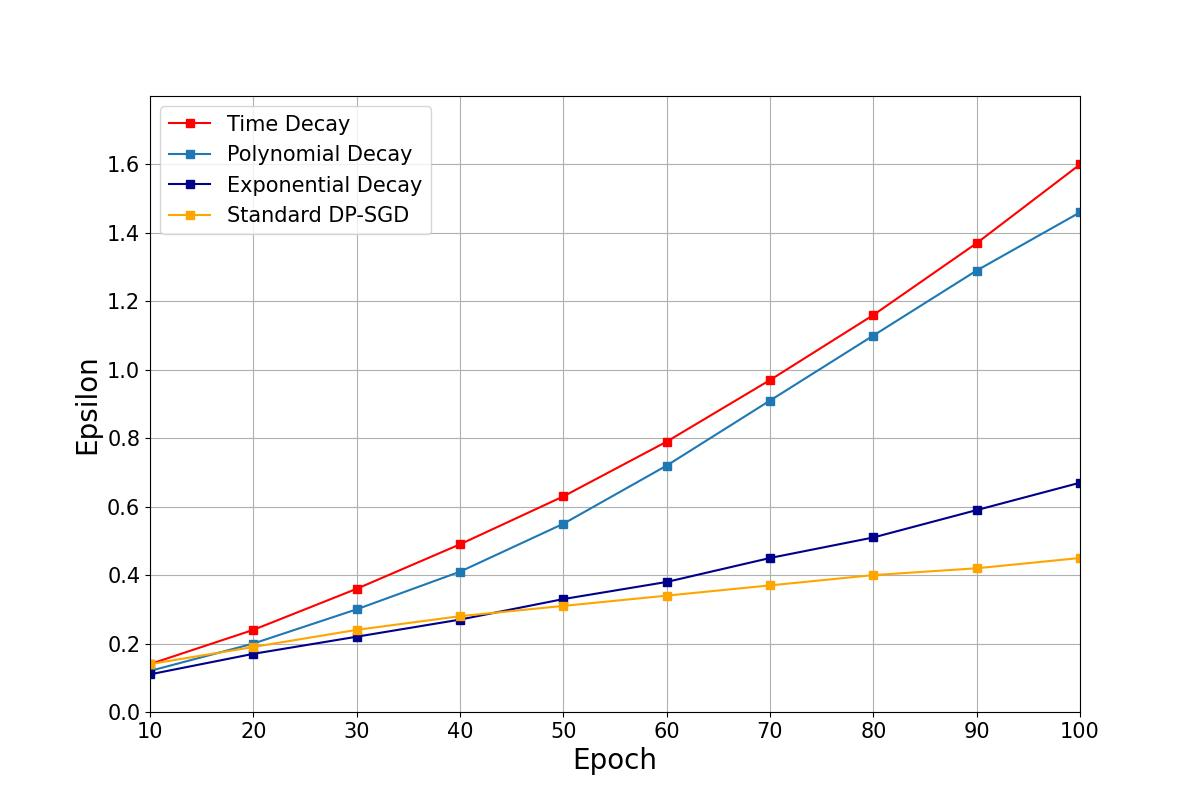
\includegraphics[width=0.7\linewidth]{submissions/submission5/figs/epsDecay.jpg}
   \caption{Adaptive Privacy Budget Consumption Rate}\label{FigDiff}
   \label{decayRate}
\end{figure} 

Next, we experimented with adapting learning rate ($\eta$) and clipping threshold ($C$), according to the methodology described in~\cite{RefWorks:RefID:38-koskelalearning} and~\cite{RefWorks:RefID:37-andrewdifferentially} (described in Sections~\ref{sec:quantile} and~\ref{sec:lr}, respectively). Noise magnitude was set at $\sigma=2.0$. 
Figure~\ref{accadapt} shows the test accuracy of each technique when training on the MNIST dataset. 
Among the three, adaptive learning rate produced the best accuracy ($91.90$\%) after consuming privacy budget $\epsilon=1.0$, while adaptive clipping achieved $85.37\%$ accuracy with overall privacy budget consumption of $\epsilon=0.83$ -- a tighter privacy guarantee than standard DP-SGD which achieved accuracy of $86.00$\% after consuming $\epsilon=1.0$. 

For comparison purpose, we tested the performance of the noise magnitude time decay methodology discussed earlier using the same parameters that have been used for the latest adaptation experiments. The noise magnitude time decay seems to be the most promising among all, as it yielded an accuracy of $92.05$\% with $\epsilon = 1.0$ in a shorter training time. 
\begin{figure}[h]
\centering
        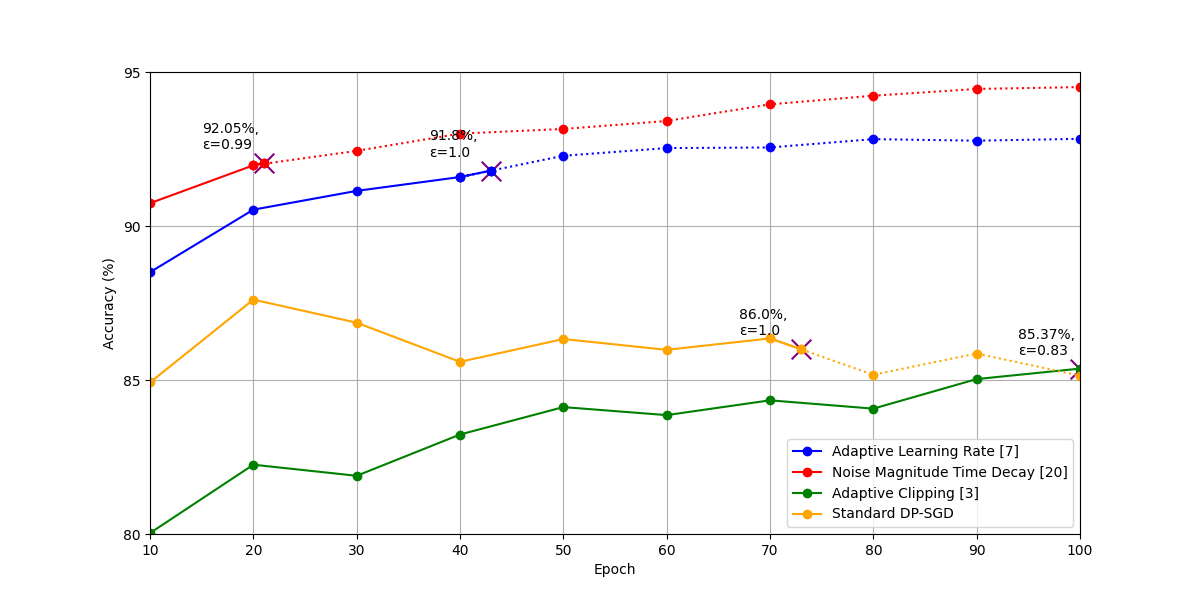
\includegraphics[width=\linewidth]{submissions/submission5/figs/AccAdapt.png}
   \caption{Accuracy of Adaptive Techniques on MNIST}
   \label{accadapt}
\end{figure} 

We conducted the same experiment on the CIFAR-10 dataset, using the same architecture and parameters used in~\cite{RefWorks:RefID:38-koskelalearning}, and $\sigma = 1.2$ for all techniques except for the exponential noise decaying approach, for which we used $\sigma_{initial} = 2.0$, in order to prevent very high privacy budget consumption. 
Figure~\ref{accadaptcifar} summarizes the results. 
Experiments on CIFAR-10 confirm the superiority of learning rate adaptation, which obtained the highest accuracy of $62.52\%$ with $\epsilon = 2.0$ going up to $64.97\%$ with $\epsilon = 3.0$. Clipping threshold adaptation produced slightly better improvements with an average of $7\%$ additional accuracy when compared to standard DP-SGD at similar privacy levels.
One important observation from this set of experiments is the performance of noise magnitude decay. Specifically, exponential noise decay is able to achieve only marginally better accuracy compared with the standard DP-SGD under similar budget consumption.

\begin{comment}
\begin{enumerate}
    \item Privacy budget consumption rate
    \item Performance improvement rate
    \item Rate of increase in the privacy budget consumption rate (resulted from the noise magnitude decay rate)
\end{enumerate}
\end{comment}

%Having a high rate of increase in the privacy budget consumption rate with a comparably high performance improvement rate can result in a better performance depending on the situation. What happened when we tried on MNIST with noise magnitude time decay is that there was a very high rate of privacy consumption but that was enough to have a higher performance improvement rate. On the other hand, CIFAR-10 is a more complicated and challenging dataset on which the performance increase is hard and need more detailed training, so what happened is that the performance improvement rate was not on the same level with the increase in the privacy budget consumption resulting in a drawback. So, in this case the choice of the noise magnitude adaptation strategy and the decay rate is very crucial along with a more powerful model architecture. In the original research \cite{RefWorks:RefID:47-yu2019differentially} they used VGG-16 architecture which reported a slight improvement with additional $2\%$ accuracy. Figure \ref{accadaptcifar} performance comparison along time on CIFAR-10 dataset



\begin{figure}[h]
\centering
        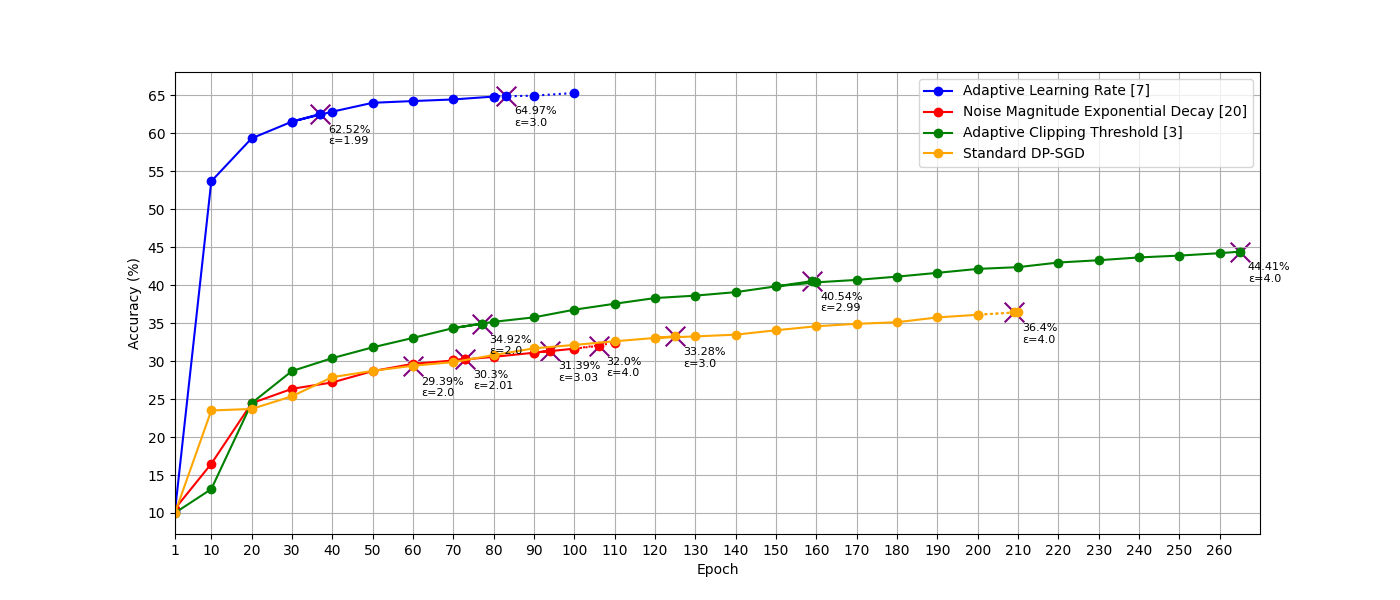
\includegraphics[width=\linewidth]{submissions/submission5/figs/AccAdaptCifar.png}
   \caption{Accuracy of Adaptive Techniques on CIFAR-10}
   \label{accadaptcifar}
\end{figure} 

\subsection{Individualized Privacy Budget Results}
We evaluate two different individualized privacy (IDP) approaches proposed by Boenisch et. al. in ~\cite{haveit}, namely {\em grouping} and {\em sampling}. We divide the training dataset into three partitions according to the privacy requirements illustrated in Table~\ref{tab: distrib}. The two distributions correspond to the settings used in~\cite{haveit} and~\cite{haveit2}, respectively. 

%A data pre-processing step is performed to extract the individualization parameters before training the model. 
First we present results obtained on the MNIST dataset. 
%with the mentioned data distribution considering the privacy budgets of Case 1 in table \ref{tab: distrib}. In our experiments, 
According to~\cite{haveit}, the sampling approach uses individual sampling rates = \{0.005, 0.009, 0.013\} for the three different privacy level groups respectively, with $\sigma_{sample}=1.368$. In the scaling approach, the corresponding individual clipping thresholds are \{0.141, 0.236, 0.299\} with $\sigma_{scale}=1.545$. After training the model using both approaches, scaling obtained accuracy of $97.63$\% while sampling achieved $96.79$\% accuracy, both outperforming previously mentioned DP-SGD related approach. The results match the ones presented in the original IDP work from~\cite{haveit}.

We also investigated results on CIFAR-10, which were not reported previously. We include two more extreme cases of privacy requirements, cases 2 and 3 in Table~\ref{tab: distrib}. Case 1 is the only one used in the original work from~\cite{haveit}. The second case has a more pronounced variability in privacy concerns, with one group having very tight privacy requirements, while the others are more loose. Finally, the third case has two groups with relatively tight privacy requirements, and a third with almost no privacy concerns. 

Figures~\ref{sampleEps} and~\ref{scaleEps} show the privacy consumption rates for each group in case 1. As shown in Figure~\ref{accidpcifar} and Table~\ref{tab: accIDP}, both grouping and sampling approaches were able to deal with the extreme cases, with the scaling approach giving better performance in cases 2 and 3. The most extreme cases lead to slowest convergence in training. This is a result of overfitting, as the sampled examples originate mostly in group 3, and thus the model finds it difficult to generalize results to less seen examples in groups 1 and 2. 

\begin{table}[!htp]\centering
\caption{Individualized Data Distributions}\label{tab: distrib}
\scriptsize
\begin{tabular}{|p{1.7cm}|p{1.7cm}|p{1.7cm}|p{1.7cm}|p{1.7cm}|}\toprule
\hline
\textbf{Group \#} &\textbf{Percentage of Data} &\textbf{Case 1}&\textbf{Case 2}&\textbf{Case 3}\\\midrule
\hline
\textbf{Group 1 (High Privacy)} &34\% &$\epsilon = 1.0$ &$\epsilon = 1.0$&$\epsilon = 1.0$\\
\hline
\textbf{Group 2 (Medium Privacy)} &43\% &$\epsilon = 2.0$&$\epsilon = 10.0$&$\epsilon = 2.0$ \\
\hline
\textbf{Group 3 (Low Privacy)} &23\% &$\epsilon = 3.0$ &$\epsilon = 20.0$&$\epsilon = 20.0$\\
\hline
\bottomrule
\end{tabular}
\end{table}


\begin{figure}[htbp]
  \centering
  \begin{minipage}[b]{0.45\textwidth}
   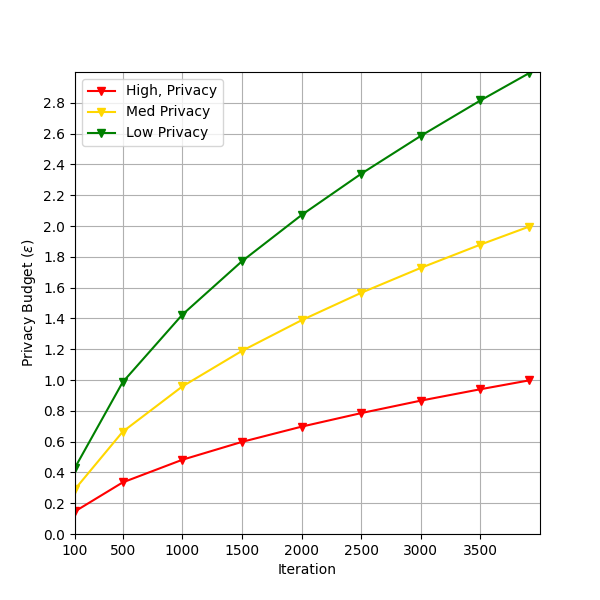
\includegraphics[width=\linewidth]{submissions/submission5/figs/epsindividone.png}
   \caption{Individualized privacy budget consumption over time (Sampling)}\label{FigDiff}
   \label{sampleEps}
  \end{minipage}
  \hfill
  \begin{minipage}[b]{0.45\textwidth}
    \centering
    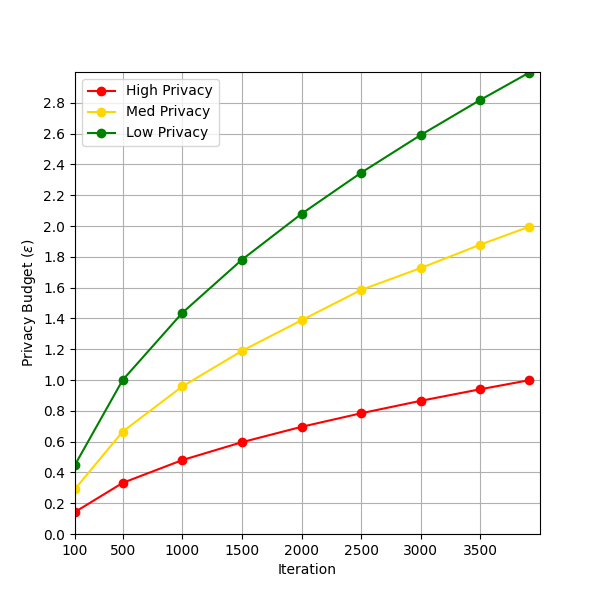
\includegraphics[width=\linewidth]{submissions/submission5/figs/epsindivid2.png}
   \caption{Individualized privacy budget consumption over time (Scaling)}\label{FigDiff}
   \label{scaleEps}
  \end{minipage}
  
\end{figure}

\begin{table}[!htp]\centering
\caption{Performance of IDP-SGD on CIFAR-10}\label{tab: accIDP}
\scriptsize
\begin{tabular}{|p{1.7cm}|p{1.7cm}|p{1.7cm}|p{1.7cm}|p{1.7cm}|}\toprule
\hline
\textbf{Approach}  &\textbf{Case 1}&\textbf{Case 2}&\textbf{Case 3}\\\midrule
\hline
\textbf{Sampling}  & 59.03\% & 59.49\% & 59.7\% \\
\hline
\textbf{Scaling} & 58.26\% & 67.64\% & 63.07\% \\
\hline
\bottomrule
\end{tabular}
\end{table}
\begin{figure}[h]
\centering
        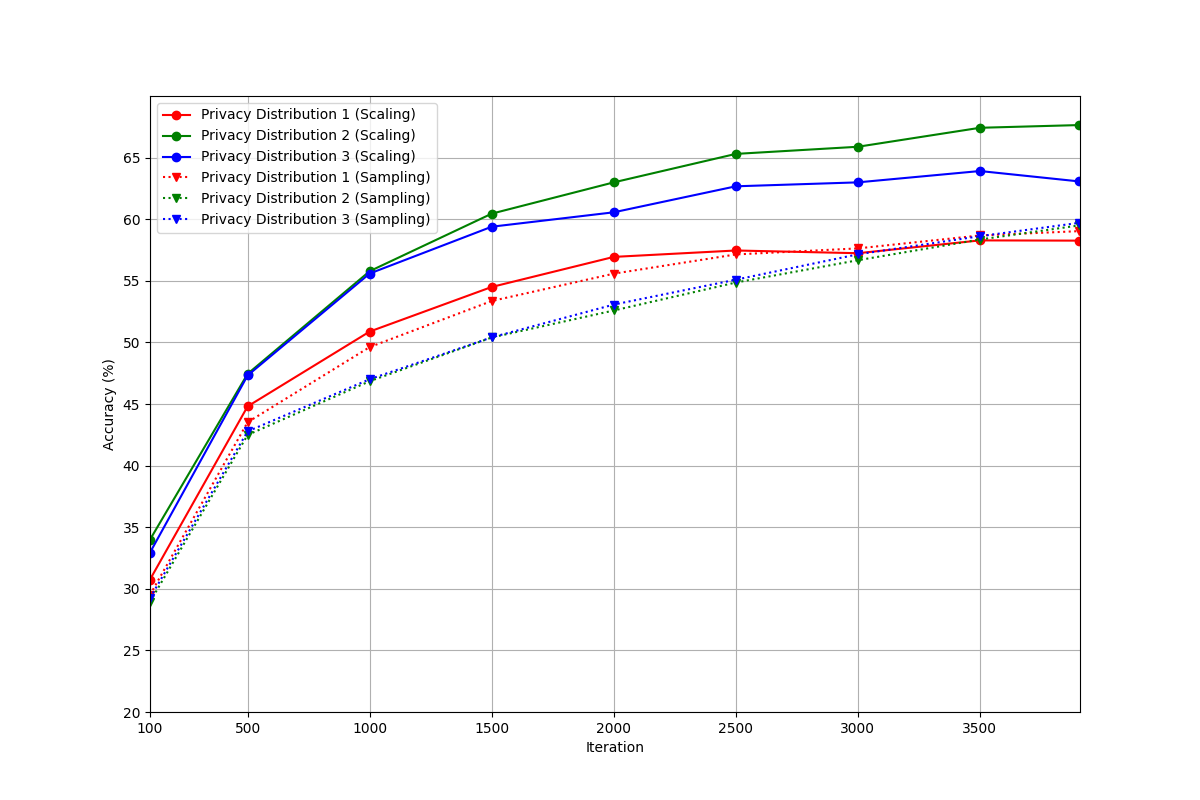
\includegraphics[width=\linewidth]{submissions/submission5/figs/cifarindivid.png}
   \caption{Testing accuracy for IDP-SGD techniques on CIFAR-10}\label{FigDiff}
   \label{accidpcifar}
\end{figure} 


\section{Conclusions}
\label{sec:conclusions}

In this article, we reviewed several categories of prominent DP-SGD techniques with respect to several criteria, such as strategies for adaptive hyperparameter tuning, data management considerations, and individualized privacy requirements. With the current advent of machine learning in virtually all application domains, DP-SGD is expected to become increasingly deployed in practice. Therefore, it is important to understand well its privacy-accuracy trade-off, its underlying influential factors, and how to adapt private learning to obtain a good compromise between protection, accuracy and performance. In future work, we plan to extend our review to techniques for private learning in large language models, which present a different set of challenges, due to the multiple ways in which unstructured language from individuals can carry sensitive information into the final model.










\bibliographystyle{ieeetr}

\bibliography{submissions/submission5/sample}

\end{document}